
%----------------------------------------------------------------------------------------
%	PACKAGES AND OTHER DOCUMENT CONFIGURATIONS
%----------------------------------------------------------------------------------------

\documentclass[twoside,twocolumn]{report}

\usepackage{blindtext} % Package to generate dummy text throughout this template 

\usepackage[sc]{mathpazo} % Use the Palatino font
\usepackage[T1]{fontenc} % Use 8-bit encoding that has 256 glyphs
\linespread{1.05} % Line spacing - Palatino needs more space between lines
\usepackage{microtype} % Slightly tweak font spacing for aesthetics

\usepackage[english]{babel} % Language hyphenation and typographical rules

\usepackage[hmarginratio=1:1,top=32mm,columnsep=20pt]{geometry} % Document margins
\usepackage[hang, small,labelfont=bf,up,textfont=it,up]{caption} % Custom captions under/above floats in tables or figures
\usepackage{booktabs} % Horizontal rules in tables

\usepackage{lettrine} % The lettrine is the first enlarged letter at the beginning of the text

\usepackage{enumitem} % Customized lists
\setlist[itemize]{noitemsep} % Make itemize lists more compact

\usepackage{titlesec} % Allows customization of titles
%\renewcommand\thesection{\Roman{section}} % Roman numerals for the sections
%\renewcommand\thesubsection{\roman{subsection}} % roman numerals for subsections
\titleformat{\section}[block]{\large\scshape\centering}{\thesection.}{1em}{} % Change the look of the section titles
\titleformat{\subsection}[block]{\large}{\thesubsection.}{1em}{} % Change the look of the section titles

\usepackage{fancyhdr} % Headers and footers
\pagestyle{fancy} % All pages have headers and footers
\fancyhead{} % Blank out the default header
\fancyfoot{} % Blank out the default footer
\fancyhead[C]{\today $\bullet$ Parting the Clouds $\bullet$ 16019243} % Custom header text
\fancyfoot[RO,LE]{\thepage} % Custom footer text

\usepackage{titling} % Customizing the title section

\usepackage{pdflscape}

\usepackage{hyperref} % For hyperlinks in the PDF

\usepackage{pdfpages}

\usepackage{csquotes}

\usepackage{caption}
\usepackage{subcaption}


\usepackage[backend=biber, style=authoryear, maxnames=999, maxcitenames=3, urldate=long, natbib=true]{biblatex}
%\DeclareNameAlias{sortname}{last-first}
\DeclareFieldFormat{edition}{%
  \ifinteger{#1}
    {\ifnumequal{#1}{1}%
     {}%
     {\mkbibordedition{#1}~\bibstring{edition}}%
    }
    {#1\isdot}}

\DeclareFieldFormat[article,inbook,incollection]{title}{#1\isdot}
\DeclareFieldFormat[article,inbook,incollection]{citetitle}{#1\isdot}

\newrobustcmd{\MakeTitleCase}[1]{%
  \ifboolexpr{test {\ifentrytype{article}} or test {\ifentrytype{inbook}} or test {\ifentrytype{incollection}}}
    {#1}
    {\MakeSentenceCase{#1}}}

\DeclareFieldFormat{urldate}{\bibsentence\mkbibbrackets{\bibstring{urlseen}\space#1}}
\DeclareFieldFormat{url}{\bibstring{urlfrom}\addcolon\space\url{#1}}


\renewbibmacro*{volume+number+eid}{%
  \printfield{volume}%
%  \setunit*{\adddot}% DELETED
  \setunit*{\addnbspace}% NEW (optional); there's also \addnbthinspace
  \printfield{number}%
  \setunit{\addcomma\space}%
  \printfield{eid}}
\DeclareFieldFormat[article]{number}{\mkbibparens{#1}}


\renewbibmacro*{journal}{%
  \iffieldundef{journaltitle}
    {}
    {\printtext[journaltitle]{%
       \printfield[titlecase]{journaltitle}%
       \setunit{\subtitlepunct}%
       \printfield[titlecase]{journalsubtitle}}
       \ifboolexpr{
         not test {\iffieldundef{url}}
         or
         not test {\iffieldundef{urldate}}
         or
         not test {\iffieldundef{doi}}
         or
         not test {\iffieldundef{eprint}}
       }
         {\nopunct\bibstring[\mkbibbrackets]{online}}%
         {}}}

\renewbibmacro*{journal+issuetitle}{%
  \usebibmacro{journal}%
  \setunit*{\addspace}%
  \iffieldundef{series}
    {}
    {\newunit
     \printfield{series}%
     \setunit{\addspace}}%
  \newunit
  \usebibmacro{volume+number+eid}%
  \setunit{\addspace}%
  \usebibmacro{issue+date}%
  \setunit{\addcolon\space}%
  \usebibmacro{issue}%
  \newunit}

\NewBibliographyString{online}
\DefineBibliographyStrings{english}{%
  urlseen    = {accessed},
  online     = {online},
}
%\addbibresource{example.bib}
\renewcommand*{\nameyeardelim}{\addcomma\addspace}
\renewbibmacro{in:}{%
  \ifentrytype{article}{}{\printtext{\bibstring{in}\intitlepunct}}} % removes "In" preceding journal title
  
  

%\section*{Bibliography}
%\bibliography{biblio.bib}
%\end{document}


\DeclareBibliographyCategory{cited}
\AtEveryCitekey{\addtocategory{cited}{\thefield{entrykey}}}

\addbibresource{FYP.bib}
\nocite{*}

\newcommand{\citefirstlastauthor}{\AtNextCite{\DeclareNameAlias{labelname}{given-family}}\citeauthor}

\usepackage{multirow}


\linespread{1.25}



%----------------------------------------------------------------------------------------
%	TITLE SECTION
%----------------------------------------------------------------------------------------



\usepackage{glossaries}

\glstoctrue
\makenoidxglossaries

\newglossaryentry{BlueLight}
{
    name=blue light,
    description={Short wavelength, high-energy - usually below 550nm}
}

\newglossaryentry{flux}
{
	name=luminous flux,
	description={the perceived power of a light source, measured in lumen}
}

\newglossaryentry{lux}
{
	name=lux,
	description={the SI unit of illuminance, measured by \gls{flux} per unit area. Equivalent to $lumens/m^2$}
}

\newglossaryentry{solar}
{
	name=solar irradiance spectrum,
	description={the spectrum output by the sun as measured from the surface of the earth}
}


\newacronym{pcbs}{PCBs}{Printed Circuit Boards} 

\newacronym{cfl}{CFL}{Compact Fluorescent Lamp} 

\newacronym{morning}{DY}{Daytime}

\newacronym{afternoon}{ST}{Sunset}

\newacronym{evening}{TW}{Twilight}

\newacronym{night}{NX}{Night}

\newacronym{spd}{SPD}{Spectral Power Density}

\newacronym{sam}{SAM}{Spectral Angle Mapper}

\newacronym{cri}{CRI}{Colour Rendering Index}

\newacronym{s}{S}{Short-Wavelength}

\newacronym{m}{M}{Medium-Wavelength}

\newacronym{l}{L}{Long-Wavelength}

\newacronym{iprgc}{ipRGC}{intrinsically photosensitive Retinal Ganglion Cells}

\newacronym{rtc}{RTC}{Real Time Clock}

\newacronym{ic}{IC}{Integrated Circuit}

\newacronym{esd}{ESD}{Electro-static Discharge}

\newacronym{cct}{CCT}{Correlated Colour Temperature}

\newacronym{car}{CAR}{Cortisol Awakening Response}

\newacronym{sad}{SAD}{Seasonal Affective Disorder}



\begin{document}

\pagenumbering{roman}

\begin{titlepage}

    \begin{center}
        \vspace*{1cm}
            
        \Huge
        \textbf{Parting the Clouds: Moving Towards an Affordable Natural-Lighting Solution}
            
        \vspace{0.5cm}
        \LARGE
        16019243
            
        \vspace{1.5cm}
            
        \textbf{N. Appleton}
        
        \vspace{0.5cm}
        Supervisor: Matthew Studley
        
        BEng Robotics
            
        \vfill
            
        Designing a modular, human-centric lighting system   
        
        \pageref{Lastpage} pages; 
        \input{WordCount.sum}words \\ (main text only)
            
        \vspace{0.8cm}
            
        \Large
        Faculty of Environment and Technology\\
        UWE\\
        UFMFX8-30-3 \\
        \today
            
    \end{center}
\end{titlepage}


\begin{titlepage}
\centering
~
\vfill

\textbf{Disclaimer:}

All of the work contained in this document is solely the work of N. Appleton.

\vfill
~ \vfill
\end{titlepage}

\setcounter{tocdepth}{1}
\tableofcontents 
\clearpage \newpage

%----------------------------------------------------------------------------------------

%----------------------------------------------------------------------------------------
%	ARTICLE CONTENTS
%----------------------------------------------------------------------------------------
\pagenumbering{arabic}


\chapter{Introduction}
\label{Chap:Intro}

\setcounter{section}{-1}

\section{Let there be Light}

``\textit{God said, `Let there be light,' and there was light. God saw that the light was good, and he separated the light from the darkness. God called the light `day,' and the darkness he called `night'. And there was evening, and there was morning — the first day.}'' \textasciitilde Genesis 1:3-5.

Since the dawn of life itself, we have been exposed to the natural light of the sun, and the distinct separation of day and night. However, our modern, fast-paced lifestyle no longer allows for such long periods of time being wasted and unproductive in darkness.

As the literature reveals more and more ways in which this divergence harms our well-being, it seems that a serious re-think of our environments - and how we light them - is required.

\section{Gap in the Market}

Light has been shown to have serious ramifications on many facets of life: excess \gls{BlueLight} in the evenings causing sleep deficiency; lighting affecting lifestyle-related diseases; insufficient \gls{BlueLight} exposure being a risk factor for depression and other mood disorders; and plenty more that are discussed in chapter \ref{Chap:Lit}.

Chapter \ref{Lit:solutions} outlines why the existing products attempting to solve this problem are not appropriate, and thus why a new solution must be developed. 

\section{Aims and Objectives}

This project set out to try to develop an affordable, modular, broad-application natural lighting solution. 

\subsection{Aims}

There were 2 main aims that the device set out to achieve: 'To produce an affordable device that replicates the visual solar spectrum as closely as is feasible' and 'to validate the device by measuring the output spectra across the day'.

Initially, further aims included developing the device as a product by improving user experience through user interface, web apps, and other expanded functionality. This would have been researched using qualitative methods such as opinion surveys to assess the interest in the device in the consumer market. These aims were set out as stretch goals that could be undertaken when the two main aims had been completed.

\subsection{Objectives}

\begin{figure*}[bt]
\includegraphics[width=\textwidth]{Images/plan}
\caption{How the lockdown in England affected the objectives of the project. Reasons for the changes are discussed later in the document.}
\label{Objectives}
\end{figure*}

The objectives used to achieve the aims have been dynamic throughout the project. The initial plan of producing and testing 2 rounds of \acrfull{pcbs} before using these to validate the spectral outputs was heavily influenced by the pandemic. See Fig \ref{Objectives}.

Both N. Appleton and V. Halenka were involved in the design of the hardware, as it was a useful device for both areas of research. The success of these devices was assessed against the requirements specification (Appendix \ref{App:Req} and is discussed in chapter (REF).

One of the most important aims of the project from the beginning was the development of the simulator. This allowed for a contingency for that spectral measurements to be obtained even in the absence of physical hardware. The simulator was also used to explore the desired outputs of the device and how they could be achieved.

\subsection{Scope}

Keeping the scope of the project relatively flexible was an important factor due to the pandemic. Designing the hardware, which was scheduled to be done by February, was severely impacted by the lockdown that began on the 1st of January 2021. 

Due to the ``modular'' construction of the aims, the qualitative, product-based research and much of the usability development had to be left for future research and development. In removing these aims from the project, it allowed the primary objective to be successfully achieved.

Had the pandemic not had such a profound effect, the main aims would have likely been completed earlier, allowing for progression to the secondary research goals. However, going into the project, there was no way to know how the year would pan out. Using this dynamic scope worked very well and allowed the successful completion of the primary area of research. 



\section{Project Management}

%This project was approached in a self-led manner, with the hardware design being split across 2 projects. Weekly supervisor meetings have been held as well as meetings between N. Appleton and V. Halenka to ensure that all areas of work are on schedule.

\paragraph{AGILE Kanban}

The project was approached using a Kanban-style AGILE workflow, using the $ClickUp^{TM}$ project management software to organise tasks, subtasks, Gantt charts, meeting minutes, relevant literature and more. Using just one piece of software to organise all of this reduced the friction and chance of errors. For example, when updating Gantt charts, the Kanban boards and tasks are automatically updated to reflect these changes and vice versa.

\paragraph{Weekly meetings}
Both weekly supervisor meetings, and weekly meetings between the hardware developers took place to ensure that all areas of the project were progressing as planned. Alterations to the scheduled work could be discussed and approved at these meetings, further reducing the friction when needing feedback. Minutes of these meetings were made on the $ClickUp^{TM}$ software and copies were printed and pasted into the project logbook.

\paragraph{Logbook}
The logbook has been used as a hard-copy of all the digital documents that were produced throughout the project including interviews, requirements documentation, meeting minutes, invoices, design documentation and Gantt charts. All work has been logged to ensure data is not lost and the project could continue even in the event of the researcher being replaced. 

\paragraph{Gantt Charts}
The project plan Gantt charts were updated on a monthly basis to ensure their relevance and to take into account the most up-to-date information. These updates happened in meetings between the development team to allow timescales to be discussed before implementation. All Gantt charts are displayed in appendix \ref{App:Gantt}.

\paragraph{Time Constraints}
As with any project, there have been some strictly imposed time constraints throughout the year. Weekly supervisor meetings meant that there was always a two-way stream of information so as to put less importance on each meeting. 

It was important that the experimentation could be completed by the end date of the project, and that at least initial results could be gathered before the progress review that took place at the end of March.

\paragraph{Contingencies}
From the beginning of the project, a focus has been placed on creating effective contingencies to ensure that the main experimentations would give results. This has been especially true within a hardware-based project during the pandemic. The flexible aims have been discussed earlier, but many other contingencies were put in place. Building a simulator was a big priority to ensure that results could be gathered in the event of failure to obtain hardware.

\paragraph{Risks and Mitigation}
The project has been focused on de-risking throughout by front-loading the highest-risk tasks to ensure that, in the case of failure, objectives can still be met. For example, hardware development happened early on in the project to allow time to overcome any of the issues that arose.

This method of risk identification and mitigation proved extremely effective during the pandemic, when many of the unwanted outcomes came to pass.

The risk-assessment and resources forms have been kept up-to-date throughout the project to ensure that a safe working environment can be guaranteed. Few changes were made to these documents as the initial copies were good reflections of the risks and resources required.

\paragraph{Reflection}
The successful completion of all the main outcomes of the project is a testament to the good planning that has been observed from the beginning.

The continued planning  and de-risking, alongside the effective use of supervision, have ensured that all the primary aims were achieved within the timeframe. This, in turn, allowed the adherence to milestones and deadlines, including the progress review. Contingencies played a large role in delivery of the project, and are discussed further in chapter \ref{}.

Mitigating any potential risks through the use of the risk-assessment (Appendix \ref{App:Risk} early in the project allowed for progress to be made safely and appropriately. 

The Engineering Council's UK-SPEC has been consulted throughout the project and a spreadsheet has been kept up to date containing relevant evidence of each competency. This has helped to keep the project relevant to engineering professionalism and personal development. The logbook has been used as the main repository for all of the relevant documentation, minutes, notes and technical details. Using this, alongside $ClickUp^{TM}$ for planning tasks and time management, has streamlined the workflow, allowing for much more efficient use of time.

Overall, the management of this project has been executed excellently and, despite the pandemic, all changes to circumstance have been overcome (more in chapter \ref{}).

% UK SPEC





\chapter{Existing Work}
\label{Chap:Lit}

\section{Lighting}

\subsection{Introduction}

Many people do not realise how much time they spend in unnatural lighting conditions. In 2001, a study published in \textit{Nature} magazine found that the average American spends more than three quarters of their time inside \citep{klepeisNationalHumanActivity2001}. More recent studies have put this number as high as 90\% \citep{opiniumBritsSpend902018}, and when most buildings do not get adequate sunlight in the day, the time spent under man-made light sources can be significant. Furthermore, after dark, almost all buildings are lit artificially; very few people around the world do not spend their nights in lit environments.

\citet{falchiNewWorldAtlas2016} found that 86\% of the World's population, and 99\% of the US and European population live under ``light polluted'' skies. The world uses so much light, that one third of humanity, 60\% of Europeans, and 80\% of North Americans cannot see the Milky Way. 

\subsection{History}

It wasn't always this way. For only the most recent 1.5 million years - a blink of the evolutionary eye - have humans been able to harness the power of fire to extend the usable time of day \citep{gowlettEarliestFireAfrica2013}. It is important to note, however, that fire does not try to emulate daylight; fires lit after dark were used for cooking and as a social space \citep{gowlettDiscoveryFireHumans2016}.

This was until Michael Faraday's contributions to science allowed Davy to produce the first functional electric light: the arc lamp \citep{knightHumphryDavyScience1998}. Since that fateful day, humans' relationship with night has grown increasingly distant. In 1878, Swan presented the first  incandescent lamp, patented by Edison in 1880 (though it is believed that others were developing this technology concurrently) %\citep{montoyaIndoorLightingTechniques2017}
. These bulbs are very inefficient; the peak wavelength is determined by the temperature of the gas in the bulb. In order for visible emission to occur, very high temperatures must be achieved - and still the majority of the light will be infra-red (IR) and not visible to the human eye \citep{montoyaIndoorLightingTechniques2017}.

The next widely adopted innovation was discharge lamps such as sodium lamps and fluorescent tubes, as many Correlated Colour Temperatures (CCTs) could be achieved. A \acrfull{cft} could directly replace an incandescent bulb using the same fitting.

While LEDs gained widespread popularity in the early $21^{st}$ century \citep{matsumotoMeasuringHouseholdAbility2020}, the first visible light LED was produced back in 1962 by Nick Holonyak \citep{holonyakCOHERENTVISIBLELIGHT1962}, based on the even earlier LEDs of Oleg Losev from 1927 \citep{zheludevLifeTimesLED2007}. It wasn't until 1995 that a non-red LED was produced, solving the issue of monochromasity of LED technology (it was blue) \citep{nakamuraInGaNAlGaNBlue1995}.

Once white LEDs could be produced, it led to the ``Third Revolution'' of indoor lighting \citep{montoyaIndoorLightingTechniques2017}, and now LEDs are ubiquitous in modern life. New LED technology continues to be developed, such as the Organic LED (OLED), which is cheaper and offer better colour rendition. OLED technology has only recently been applied to indoor lighting \citep{phelanOLEDLightingHits2018}, although there are some promising developments in the field \citep{benderSolidStateLightingConcise2015}. However there is still some way to go before OLEDs replace LEDs in artificial lighting technology.

\subsection{Energy Consumption and Environmental Considerations}
\label{sec:Energy}

Incandescent bulbs are not efficient. in fact, they are banned from being sold in the EU because they are so inefficient \citep{euDirective2012272012}. However, this does not mean they are all bad, they actually have many benefits: firstly, they produce light much more similar to firelight than modern lighting; they are also not hazardous, something which cannot be said for fluorescents and LEDs, which also require higher resource depletion to create \citep{limPotentialEnvironmentalImpacts2013}. But LEDs use 85\% less energy and last 50 times longer than incandescents \citep{mottierLEDLightingApplications2010}. This is significant when considering that 20\-40\% of most buildings' power consumption is from lighting alone \citep{perez-lombardReviewBuildingsEnergy2008}, accounting for as much as 10\% of all power consumed in Europe \citep{bertoldiEnergyEfficiencyStatus2012}. Considering  this, and that LEDs can theoretically convert 100\% of electrical energy to visible light (thermal regulation is key) \citep{jordanChallengesLEDPackaging2012}, it is clear why the wide-scale adoption of LED technology has been so rapid \citep{matsumotoMeasuringHouseholdAbility2020}.



\section{Circadian Rhythms}
\label{sec:Circadian}

\subsection{What is the Circadian Rhythm?}

In 1729, the French scientist Jean-Jacques d'Ortous de Mairan	used plants kept completely in the dark to determine that their diurnal cycles were not caused by external light stimulus, but rather were regulated by some endogenous (internal) clock \citep{demairanObservationBotanique1729}. 

\begin{figure}
	\includegraphics[width=0.5\textwidth]{Images/KleitmanCave}
	\caption{Nathaniel Kleitman (foreground), donning an impressive beard, measures the sleep of  Bruce Richardson \citep{universityofchicagophotographicarchiveKleitmanNathanielPhotographic}.}
	\label{Fig:Cave}
\end{figure}

Amazingly, it wasn't until 1938 that someone repeated this experiment on humans. Dr. Nathaniel Kleitman was a professor of of Physiology at University of Chicago who was later to discover Rapid-Eye Movement (REM) sleep; he is known as the father of sleep research. Together with his PhD student, Bruce Richardson, and a pair of metal beds, they descended into Mammoth Cave in Kentucky for 32 days without any natural lighting stimuli. They found that their sleep-wake cycle did not corrupt into sporadic bouts of sleep, but rather stayed at a periodic length of around 26 hours, undeniably longer than the 24 hour day. This showed that humans have an internal time-keeping system that lasts about (\textit{circa}) one day (\textit{dian}); they named it the circadian rhythm \citep{kleitmanSleepWakefulness1987}.

\citet{siffreTime1964} repeated this experiment, delving himself into a cavern for 2 months, and discovered much the same results. Meanwhile, \citet{vonaschoffSpontanperiodikMenschenBei1962} kept participants in a sealed cellar for 8-19 days, also discovering a circadian rhythm of over 25 hours.

As circadian rhythms are not 24 hours long, they need to be synchronised daily, and thus must rely on a periodic stimulus to entrain them, ie. to keep them synchronised with the 24 hour day. There were 5 factors that were thought could contribute to this entrainment of the circadian rhythm, as shown in Table \ref{Tab:Factors}.

\begin{table}
\caption{The 5 potential factors for circadian entrainment \citep{czeislerEntrainmentHumanOrcadian1981}}
\label{Tab:Factors}
\begin{tabular}{l l}
\hline
 & \textit{Factor} \\
\textbf{I.}& Knowledge of time of day \\
\textbf{II.}& Light Dark cycle \\
\textbf{III.}& Social Contacts \\
\textbf{IV.}& Timing of food availability \\
\textbf{V.}& Scheduling of bed rest and activity \\
\hline
\end{tabular}
\end{table}


Factor \textbf{I} (knowledge of time) was shown to be insignificant \citep{millsCircadianRhythmsThree1964}. Factor \textbf{II} (light-dark cycles) is the most powerful in many animals and plants, but \citet{aschoffHumanCircadianRhythms1971} concluded that this effect was too weak in humans, and that factor \textbf{III} (social cues) must be our central stimulus, or zeitgerber. 

However, when inspecting the facilities used for these experiments, \citet{czeislerEntrainmentHumanOrcadian1981} realised that the researchers ``\textit{permitted the subjects to use kitchen, bathroom, bedside and desk lamps as sources of self-selected light during the `dark' phase of each cycle}'', prompting a reassessment of the role of light in the entrainment of human circadian rhythms, concluding that light-dark cycles have a ``\textit{direct synchronising effect}'' on human circadian rhythms. They then went on to publish the landmark study titled \textit{Bright light resets the human circadian pacemaker independent of the timing of the sleep-wake cycle} \citep{czeislerBrightLightResets1986}.

\subsection{Melatonin and Melanopsin}

The circadian rhythm is controlled by a part of the brain called the Hyperthalimus \citep{stephanCircadianRhythmsDrinking1972}. Specifically, in the Suprachiasmatic Nucleus (SCN), located above the optic nerve \citep{welshIndividualNeuronsDissociated1995}. The SCN sends signals to the pineal gland \citep{cassoneMelatoninRoleVertebrate1998, borjiginPINEALGLANDMELATONIN1999} which is responsible for the production and regulation of melatonin.\footnote{
There is much intrigue and mystery around the pineal gland, with many believing that it is where conciousness is generated in the brain \citep{bobMelatoninConsciousnessTraumatic2008}. Ren\'e Descartes referred to the pineal gland as the ``seat of the soul'' \citep{lokhorstDescartesPinealGland2020}.
}

Melatonin is known as the sleep hormone, or to some: the ``chemical expression of darkness'' \citep{reiterMelatoninChemicalExpression1991}, and builds up throughout the evening and is essential for sleep onset \citep{arendtImportanceRelevanceMelatonin2003}.

In 2000, a novel Opsin was found in the human eye \citep{provencioNovelHumanOpsin2000}. An opsin is a light-sensitive protein that exists in the visual cells in the eye and is what converts the energy from photons of light into electrical signals that are sent to the brain \citep{terakitaOpsins2005}. It was soon discovered that the action spectrum of this new opsin, malanopsin, did not match any of the action spectra of the known visual cells (rods and cones), implying there was a new cell that we were not yet aware of \citep{thapanActionSpectrumMelatonin2001}.\footnote{
Interestingly, melanopsiin has been found to be much more similar to invertebrate opsins than they are to visual mammalian opsins \citep{provencioMelanopsinOpsinMelanophores1998}. This, as well as the fact almost all animals produce melatonin, shows it is a truly ancient part of our biology \citep{daviesEvolutionFunctionMelanopsin2014}.
} 
This cell was found to be the \acrfull{iprgc} \citep{bersonPhototransductionRetinalGanglion2002}, the signals from which are what keeps the SCN entrained, but to not contribute to conscious vision \citep{bersonPhototransductionGanglioncellPhotoreceptors2007}. This explains why some blind people have circadian rhythms that can be entrained with light, as discussed in the review by \citet{allenCircadianRhythmsBlind2019}.

\subsection{Blue Light}

It has been established that light is of great significance in circadian regulation, and that ``moderate illumination'' of around 500 lux \citep{laaksoOnehourExposureModerate1993}, or even ``room light'' of less than 200 lux \citep{gooleyExposureRoomLight2011} can cause a phase shift in the circadian rhythm. Furthermore, due to the action spectrum of the \acrshort{iprgc}, \gls{BlueLight} causes a much larger effect than longer-wavelength light \citep{lockleyHighSensitivityHuman2003}.

The effect of \gls{BlueLight} is so potent, that even one second pulses of \gls{BlueLight} through closed eyelids are enough to suppress melatonin production \citep{figueiroTrainBlueLight2013}, thereby dramatically affecting sleep. 

There are a few existing solutions attempting to tackle this problem. For example, the use of amber glasses can filter out blue wavelengths before they reach the retina, and have been shown to improve sleep when worn in the evenings \citep{kimberlyAmberLensesBlock2009}.






\section{Health Implications}
\label{Sec:Health}


In a meta-analysis, \citet{sanchez-barceloClinicalUsesMelatonin2010} discuss the potential effects of melatonin in a host of situations, including \textit{``ocular diseases, blood diseases, gastrointestinal tract diseases, cardiovascular diseases, diabetes, rheumatoid arthritis, fibromyalgia, chronic fatigue syndrome, infectious diseases, neurological diseases, sleep disturbances, aging and depression [as well as being] used as a complementary treatment in anaesthesia, hemodialysis, in vitro fertilization and neonatal care''}.

\subsection{Cancer}

We've known for a long time that total visual blindness is protective against many types of cancer \citep{hahnProfoundBilateralBlindness1991, feychtingReducedCancerIncidence1998, flynn-evansTotalVisualBlindness2009}. It has also been observed in many studies that flight attendants are more likely to develop breast cancer, as summed up in the meta-analysis by \citet{tokumaruIncidenceCancerFemale2006}. This effect was also observed in night-shift workers, shown in two large reviews of the existing evidence \citep{kolstadNightshiftWorkRisk2008, stevensLightatnightCircadianDisruption2009}. It is also known that the circadian rhythm has a cancer-suppressing effect \citep{fuCircadianClockPacemaker2003} and that circadian disruption is a promoting factor for lung cancer \citep{papagiannakopoulosCircadianRhythmDisruption2016}. An extensive meta-analysis even found that chemotherapy toxicity correlates to when it is taken, leading to the entire field of chronotherapy \citep{focanCircadianRhythmsCancer1995, dallmannChronopharmacologyNewInsights2014}.

The correlation of circadian regulation and cancer is so well recognised that even the WHO classes night-shift work as a class 2A carcinogen \citep{whoBreastCancerConundrum2013}. However, even those not engaging in abnormal working hours may have an increased risk; \citet{stevensBreastCancerCircadian2014} blames electric lighting directly as the cause of breast cancer being the leading cause of cancer death among women worldwide.


\subsection{Diabetes}

Although 415 million people worldwide live with Type II Diabetes, it is a preventable and reversible disease \citep{fungDiabetesCodePrevent2018}. Type II diabetes is a lifestyle disease, mostly caused by diet, whereby insulin resistance is built up such that blood sugar can no longer be absorbed by cells. A contributing factor to this is melatonin, which has been shown to aid blood glucose homoeostasis \citep{bouatia-najiVariantMTNR1BAssociated2009}. Melatonin receptors influence fasting glucose levels \citep{prokopenkoVariantsMTNR1BInfluence2009} and when completely removed, can even induce insulin resistance \citep{contreras-alcantaraRemovalMelatoninReceptor2010}.

Another study found that social jetlag - the jetlag-like effect of inconsistent waking times, ie. waking up later at the weekend - is a risk factor for obesity, itself the largest risk factor for Type II Diabetes and a host of other health issues \citep{roennebergSocialJetlagObesity2012}

\subsection{Seasonal Affective Disorder}

Seasonal Affective Disorder (SAD) is caused by a lack of light in the winter months when the sun is lower and takes a shorter path across the sky \citep{eastmanNaturalSummerWinter1990}. It has been long considered a fact that bright light helps alleviate the symptoms of SAD \citep{magnussonTreatmentSeasonalAffective1991, leeSpectralPropertiesPhototherapy1997,eastmanBrightLightTreatment1998}, but this has actually been quite a controversial topic, with others claiming that the placebos in these studies were not adequate, and that the anti-depressant effect can be attributed to placebo effect \citep{eastman26ComparisonTwo1993}. A comprehensive meta-analysis found that only 13\% of studies published between 1975 and 2003 were adequate in their methods \citep{goldenEfficacyLightTherapy2005}. The meta-analysis also highlighted the importance of dawn simulation, which performed better than both bright-light and placebo effects significantly \citet{averyDawnSimulationBright2001}.


\section{Cortisol and Attentiveness}
\label{Sec:Cortisol}

Melatonin is essential for sleep, building throughout the evening and peaking in the middle of the night. Similarly, Cortisol - produced in the adrenal gland - helps us wake up, and peaks around mid-morning. This is known as the Cortisol Awakening Response (CAR) and is, of course, also regulated by the circadian rhythm \citep{friesCortisolAwakeningResponse2009}.

Cortisol is the hormone of wakefulness and alertness and it has been shown that a higher spike in morning cortisol is correlated with better cognitive performance \citep{evansDiurnalCortisolCycle2011}, and general daytime cortisol improves alertness \citep{chapototCortisolSecretionRelated1998}. It is clear, then, that we want to maximise the CAR, which can be done through exposure to short-wavelength (blue) light after awakening \citep{figueiroShortWavelengthLightEnhances2012}. Dawn simulation has also been shown to improve the CAR - more so than just \gls{BlueLight} - as well as improving melatonin regulation, increasing well-being, mood and cognitive performance \citep{gabelEffectsArtificialDawn2013}.

It is also well documented that cortisol is a large contributing factor to mood disorders, especially bipolar disorder \citep{youngCortisolMoodDisorders2004}. A study by \citet{sitLightTherapyBipolar2007} found that \textit{``Women with bipolar illness are highly sensitive to morning bright light treatment''}, following this up a decade later with a double-blind placebo controlled trial that found that 68.2\% of the bright light participants had their bipolar disorder go into remission, compared with only 22.2\% in the placebo group \citep{sitAdjunctiveBrightLight2017}.

\section{Mood and Lighting}

Lighting arrangements affect how we perceive spaces \citep{durakImpactLightingArrangements2007}, with the general finding being that daylight-style LEDs are the most comfortable during daytime hours \citep{cajochenEffectDaylightLED2019}. It is also known that red ambient lighting is more relaxing than blue \citep{lauferPsychophysiologicalEffectsColoured2009}, and that blue causes more stimulation that red \citep{schweitzerInvestigationGenderAgerelated2016}. Pulsating orange light has also been shown to be even more relaxing \citep{wanInfluenceLightingColor2012}, it seems as though this could have a link to the fact it is a closer approximation to firelight.

Full-spectrum lighting has been thought to improve cognitive performance and mood states \citep{berryWorkEfficiencyMood1984}. However, this is somewhat controversial and likely to be a placebo effect \citep{veitchDemandCharacteristicsFull1991}.

\begin{figure}[t]
\centering
\LARGE
\textbf{``Light affects our sleep more powerfully than any drug''}

\citep{czeislerPerspectiveCastingLight2013}
\end{figure}


\section{Summary of Literature}
\label{sec:LitSummary}

Over the past 150 years, electric lighting has gone from a pipe-dream to an everyday necessity, increasing the length of the productive day. 

Alongside these developments, circadian science has been driving forward, from observations of the nature of free-running circadian rhythms to the discovery that light has profound affects upon them. \Gls{BlueLight}'s effect is especially powerful and is becoming more and more ubiquitous as our technology advances. As \citet{czeislerPerspectiveCastingLight2013} says in his landmark perspective piece entitled \textit{Casting the Light on Sleep Deficiency: ``Technology has effectively decoupled us from the natural 24-hour day to which our bodies evolved''}. 

This decoupling is dangerous for many aspects of our health. Not only is sleep important for all aspects of health and well-being, melatonin itself has a promising effect on many diseases including type II diabetes, SAD, cancer, and many others. Cortisol, melatonin's sister hormone, is also essential for a healthy life and promotes attentiveness, alertness and cognitive function.

Looking to the past for answers, we see that the output spectra of more outdated technologies such as incandescent bulbs are far more appropriate for evening use than the more modern fluorescent tubes and LEDs. But these older technologies are far less energy efficient. On the other hand, the adoption of more energy efficient technologies should not come at the expense of human health \citep{boyceReviewImpactLight2010} due to excessive \gls{BlueLight} exposure - which has also been shown time and again to damage our eyes in excessive quantities \citep{uedaEyeDamageControl2009, kuseDamagePhotoreceptorderivedCells2014, niwanoBlueLightInjures2014, marekBlueLightPhototoxicity2018, nakamuraExposureExcessiveBlue2018}.

\Gls{BlueLight} is not all bad, though. Its effects on SAD, bipolar disorder, and cognitive ability show that it is all about giving our body the right light at the right time of day. Some people already strive for this by using \gls{BlueLight} blocking glasses or RGB LED bulbs that can be set to change colour. These technologies are flawed, though: glasses are an inconvenience to wear and RGB LEDs only approximate perceived colours by combining red, green and blue, thereby ensuring there is more short-wavelength light that is desirable \citep{gilewskiEcologicalHarmfulnessRGB2018}.

This has led many to believe that an overhaul in the lighting used in the built environment is of paramount importance, with many papers calling for immediate action \citep{webbConsiderationsLightingBuilt2006, boyceReviewImpactLight2010, groseArtificialLightNight2014}.




\section{Existing Solutions}
\label{Lit:solutions}

An analysis of existing solutions was undertaken early in the project to understand what already exists in this field. The products could be generalised into 4 categories:

\subsection{Wake-Up Lights}

Ranging from £20 to £200, these products usually come in the form of an alarm clock with a built in light to wake up the user with a simulated dawn. With many varying features across the models, most contain an FM radio.

These lamps are used as a bedside light and are not appropriate for lighting a whole space. As they are focused on morning light, many use inappropriate spectra to be used before going to sleep.

 While these devices utilise an artificial dawn - shown to have many beneficial effects - there are few studies on these devices themselves.

\subsection{Bulb Replacements}

Various forms of smart-light exist on the market currently, most notably the Philips Hue. this can be set to fade to warmer light in the evenings and brighter light during the day to encourage winding-down and focus respectively. 

However the basis of these are very much visual entertainment, not circadian entrainment. Using RGB LEDs, they are less than ideal for use before bed and need serious modifications to automatically change temperature.

These bulbs are expensive, too.  For a starter kit including the base unit and just 4 bulbs, Philips charge almost £200.

Circadian bulbs also exist. These are fitted to dimmer circuits and change temperature instead of dimming. BIOS lighting have a natural spectrum bulb that can be used both in day and night. However, these require manual adjustment throughout the day and require dimmer circuits to be installed.

\subsection{Industrial Circadian Lighting}

There are many companies offering bespoke services to fit circadian lighting systems into office spaces and warehouses. However these are very expensive and not appropriate for home installation. Furthermore, as they are designed for business environments, many of these solutions do not account for later evening light that can aid with sleep onset.

\subsection{Software Based}

Windows, OSX, iOS and Android all now have built in \gls{BlueLight} filters that can be turned on to limit the amount of \gls{BlueLight} that the screen emits. The intensity and time that it comes on can usually be adjusted by the user. Specialist software such as f.lux can also be used for this purpose but with greater flexibility.

\subsection{Discussion}

All of the devices discussed here have one other feature in common: as they are all LED devices based on providing a visual cue and are not designed based on the evidence in the literature at the forefront (perhaps with industrial solutions as the exception), the spectra of these devices can be questionable.

Also, none of these products are designed to become dim enough to be used late at night. They are all for use leading into the evening, but once the user is in bed, these become insufficient solutions.

\section{Implementation}

The ideas discussed in this chapter were used to inform the requirements specification (Appendix \ref{App:Req}). The output spectra of the lamp will have to be respectful of biological considerations: no light produced within the melanopsin action spectrum during the evening, but high \gls{BlueLight} in the morning. Dawn simulation must be achievable on the device to gain many of the benefits.

The existing solutions have shown that the device must be low cost, and fully automated to bridge all of the shortcomings of the current devices. The device should also be simple to install and not require additional technology such as a smartphone.


\chapter{Methods}

There were 3 major phases to the project: idea generation, project setup, development and research. Each of these phases was approached in a different way in acknowledgement of the differences of each phase.

\section{Idea Generation}






\chapter{Results}
\label{Sec:physicalOuts}

\section{Device}

The main physical output of this project has of course been the device itself, which has already gone through a few iterations just in this short year.

\subsection{Initial Designs}

The schematic design for the device was done in KiCAD, an open-source electronics design software suite. This was chosen due to familiarity and the flexibility for adding components that are not built in. There are also extensive libraries, including a DigiKey library that adds many of the parts stocked by DigiKey for ease of design.

These designs were then laid out into prototype \acrshort{pcbs} that were ordered through JLCPCB for economical production, including pick-and-place of the surface-mount components. These \acrshort{pcbs} were designed with the USB and LED modules connected to the main board with mouse-bites, to allow for them to be snapped off after testing. This way the prototype board could be conveniently connected to all the required parts for testing, then could be snapped into its component parts for more accurate modelling of the final product. These snappable daughter boards could be reconnected to the main board via pin headers for each of the required connections, meaning they could be mounted directly back on to the main board, or connected via wires at a distance (in a more similar way to how the final product would function). 

\begin{figure}[bt]
\centering
\includegraphics[width=0.45\textwidth]{images/pcb3d1.png}
\caption{3D render of the first set of \acrshort{pcbs} created in KiCAD. Top right is the snappable LED module, the USB programmer is on the bottom right snappable daughter-board.}
\label{Fig:PCB1}
\end{figure}

Unfortunately, due to England's national lockdown, this round of \acrshort{pcbs} could not be retrieved and were returned to JLCPCB. This meant that alternative action had to be taken. Furthermore, due to the University's policy on soldering at home during the lockdown, they would not have been able to be completed either way.

\subsection{Breadboard}

For this reason, an alternative approach was required. A solderless breadboard was acquired and breadboard-friendly components were ordered. A breadboard prototype was then produced from the original schematics, as shown in Figure \ref{Fig:breadboard}.

An ESP32 board was required to ensure that the main function would be the same as the schematics. The Feather Huzzah32 from Adafruit was a board using the same programming chip (CP2104), as well as having the ESP32 and an optional ``wing'' that could add the PCF8523 \acrfull{rtc} and a micro-SD card slot, much the same as that on the schematic.

\begin{figure}[tb]
\centering
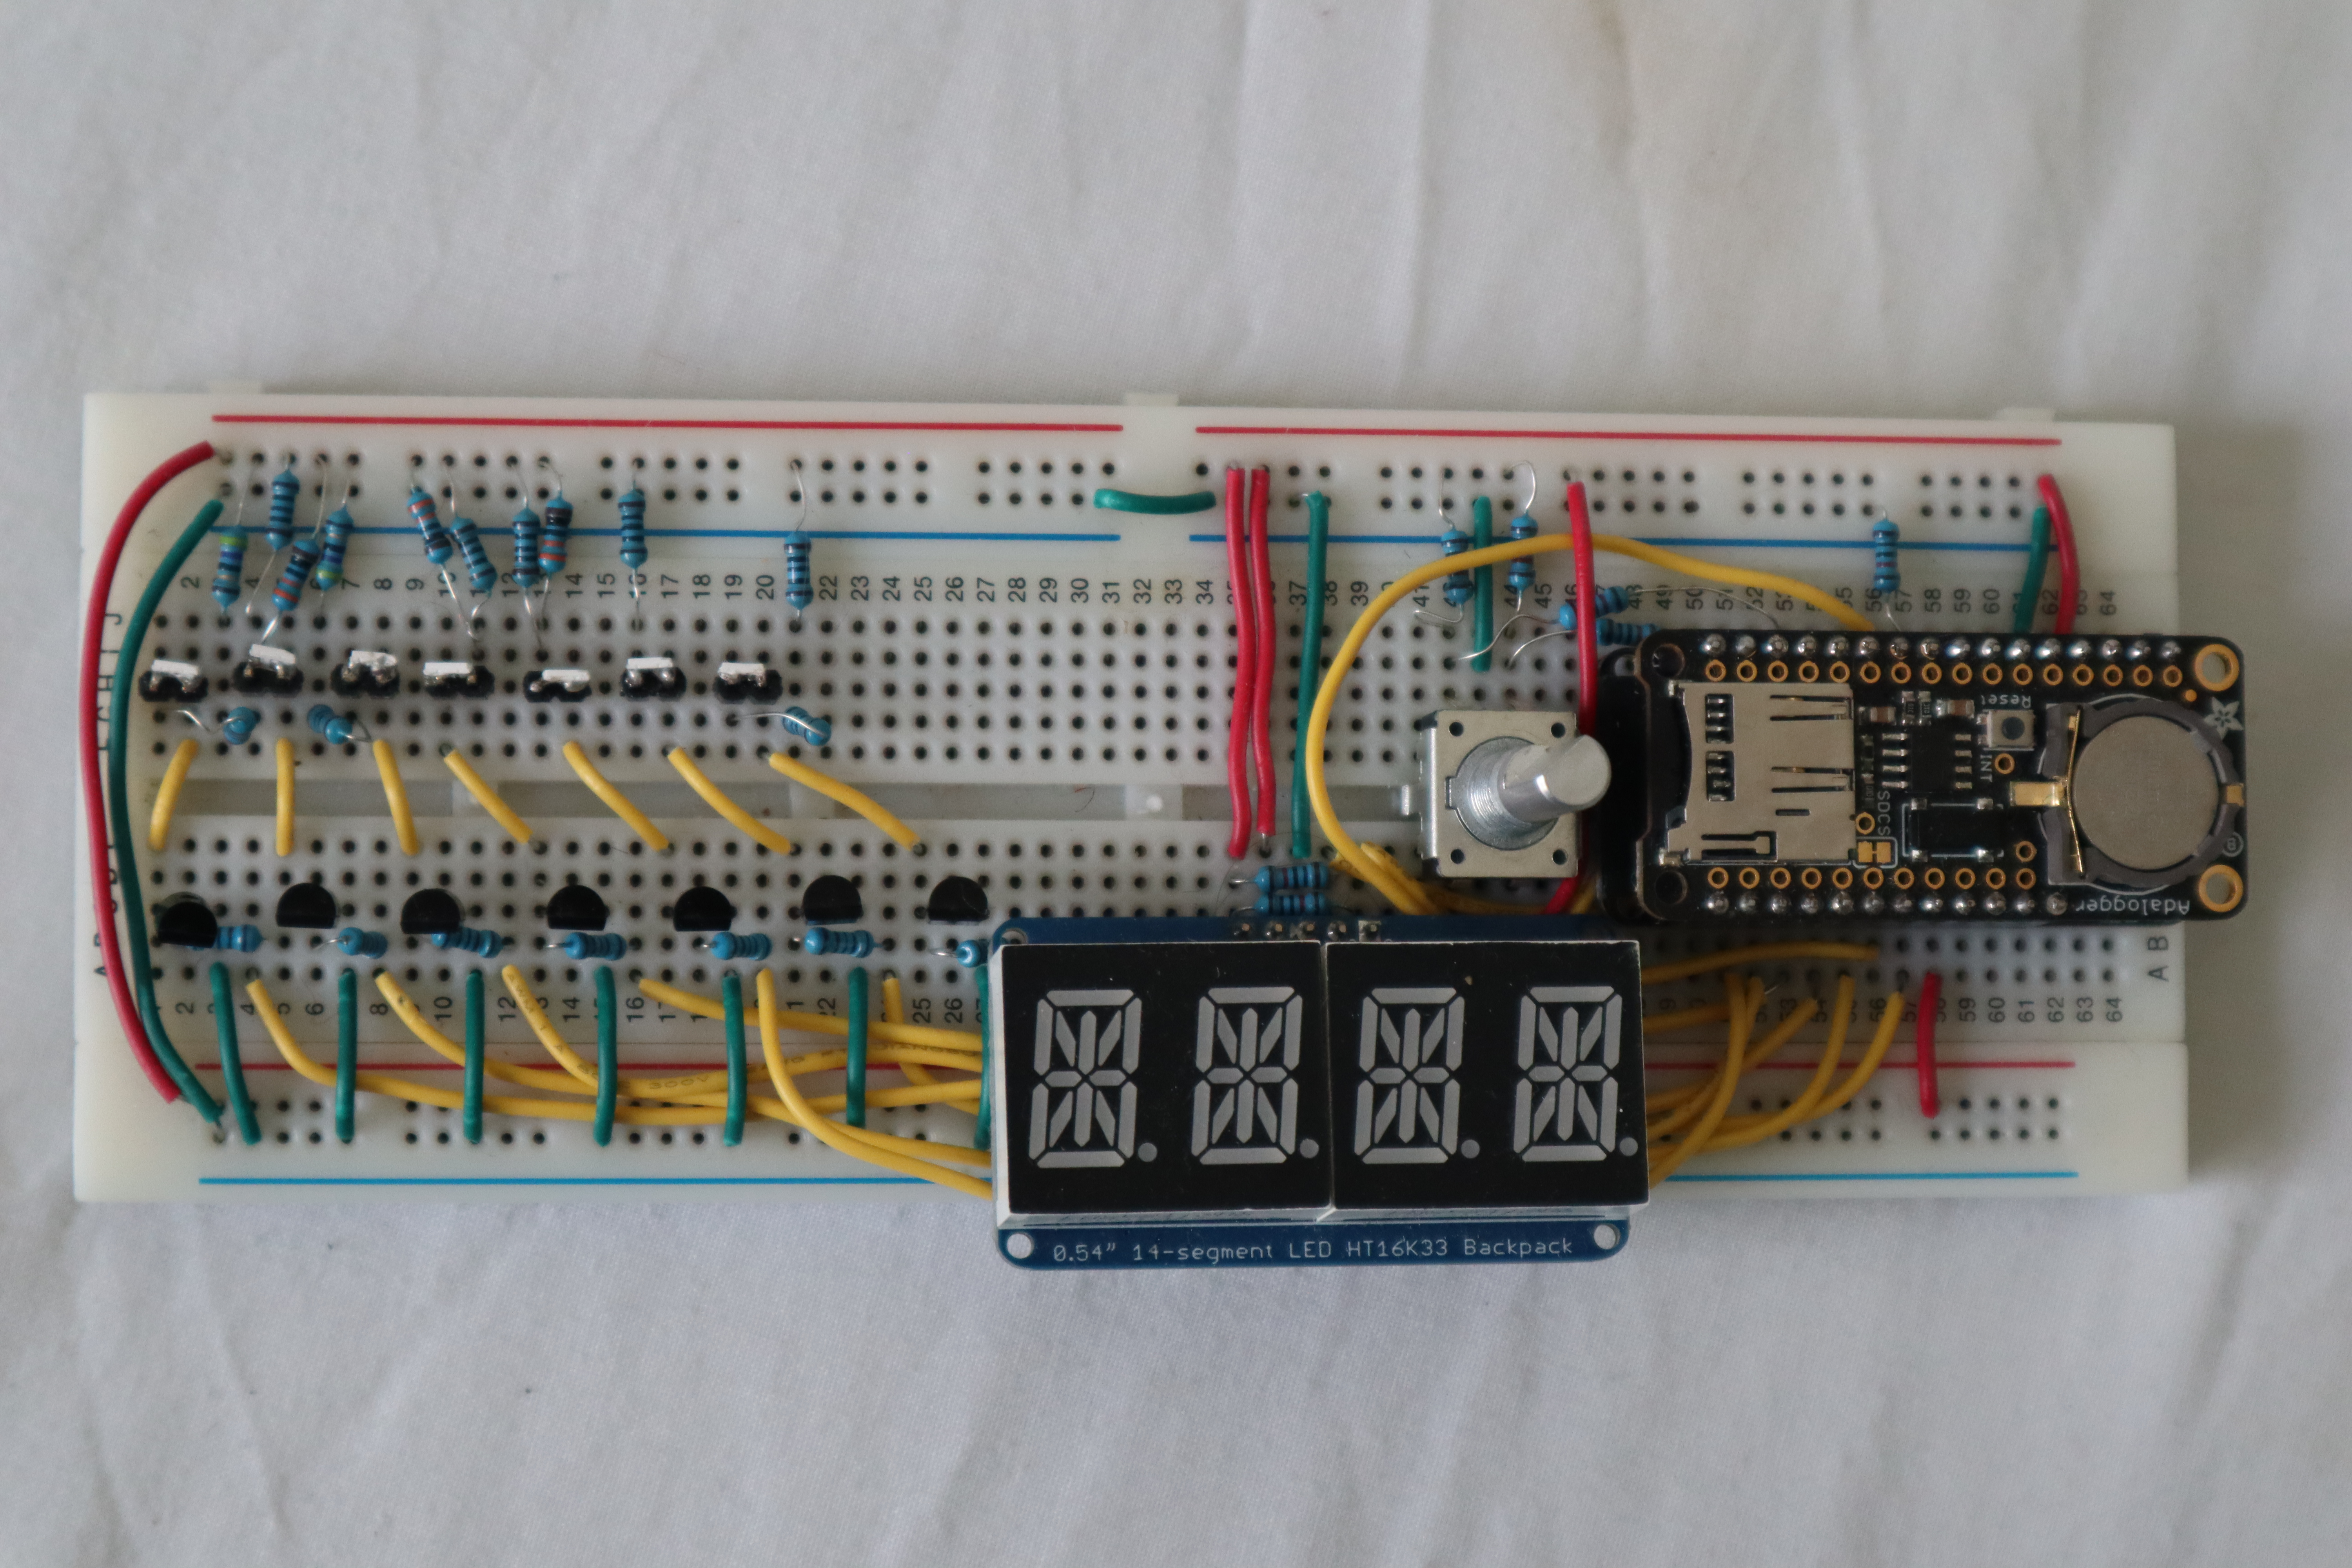
\includegraphics[width=0.45\textwidth]{images/Breadboard.JPG}
\caption{The breadboard prototype used as a proxy for the real device.}
\label{Fig:breadboard}
\end{figure}

The same LEDs were used on the breadboard as were going to be used on the \acrshort{pcbs} so that the outputs would be the same. The other components were kept as similar as possible, with all of the through-hole components remaining the same.

\subsection{Firmware}

The prototype was programmed in the Arduino language as many libraries were available that made reading the encoder, writing to the 14-segment display, and changing the brightness of the LEDs trivial.

\subsection{Final Design}

\begin{figure}[bt]
\centering
\includegraphics[width=0.5\textwidth]{images/Concept.png}
\caption{The concept drawing of what the final controller module could look like, as imagined by a product designer.}
\label{Fig:Concept}
\end{figure}


Once it had been confirmed that the breadboard prototype functioned fully and correctly, a new set of \acrshort{pcbs} were ordered, this time with high confidence of them working. 

The boards contained programming capabilities via a micro-usb, including auto-reset functionality for ease of programming. 2 levels of power regulation were included, the 12V that would be the main input and run the LEDs, as well as a 3.3V regulator to run all of the logic circuitry.

A physical reset button was added to ensure the device could be effectively tested and debugged easily. I2C was used to communicate with the \acrshort{rtc} and the screen, and SPI was used to integrate the SD card.

All \acrshort{ic}s were decoupled with a pair of capacitors, 1nF and 100nF to improve the transient response. All external ports were also protected by 15kV \acrshort{esd} diodes. Bulk capacitors were also used to ensure smooth power supply throughout the board, which itself had 4 layers: signal, ground, power, signal.

LEDs were controlled by low-side NPN transistors to decouple them from the logic circuitry. These were mounted on a separate 2-layer board with a large ground plane on both sides to aid thermal regulation.

Both the schematics and PCB layouts can be viewed in Appendix \ref{App:Electronics}.

A product designer was also employed to create a concept drawing for how the final controller device may look if it were developed into a real product. This is shown in Figure \ref{Fig:Concept}.

\section{Simulator}

Alongside the hardware development was the production of the simulator; created in LabVIEW, it was designed to approximate the spectral output of the device to be used to develop the spectra that would be implemented without having to have constant access to the measurement facilities. The LEDs' outputs were approximated using Gaussian and bell-shaped curves, generated in custom made sub-VIs. Sliders were used for simple LED adjustment and a button allows the user to save the current spectrum as a csv file for processing. The LabVIEW code for the simulator can be viewed in Appendix \ref{App:Sim}.

The simulator was calibrated using actual measured spectral outputs from the device, with each LED output being individually tuned first, then all combinations of LEDs being assessed and validated to ensure the interactions between colours was correct. This ensured that the simulator functioned in the same way as the device in all possible scenarios.

\section{Spectrometer}

\begin{figure}[b]
\centering
\includegraphics[width=0.45\textwidth]{images/CDDVD.jpg}
\caption{Microscope images of a CD and DVD, the DVD has much smaller pits, equating it to a higher resolution diffraction grating \citep{avsdiskcreatorAVS4YOUAVSDisc2019}.}
\label{Fig:CDDVD}
\end{figure}

Measuring the actual device was also made significantly harder due to the lockdown. Access to the hyperspectral camera was revoked in line with the stay-at-home order. An alternative method for recording the spectra had to be found. Many potential solutions were discussed with machine vision specialists, but many of the proposed solutions were not-applicable as they could not capture the entire spectrum.

A spectrometer that could achieve full visible-spectrum range was produced which could be used to gather the spectral data from the device.

This spectrometer was based on a simple slit, that directed light towards a diffraction grating that split the light into its component colours which could be captured with a camera.

For the initial attempt, a box was used with a CD as a diffraction grating and mirror, reflecting the light towards the camera. However, the camera was mounted too far away and could not pick up good images of the spectrum.

The second attempt used a transmissive approach: the mirror-like layer of the CD was removed and the camera could be put directly against it. This time the box was too small, and the slit could be seen in the frame of the image from the camera.

Finally for the third attempt - dubbed $Mk.3$ - a long tube was used as the body, so the camera could not see the slit. 2 Were produced: the reflective ($Mk.3_r$) and transmissive ($Mk.3_t$) models. The diffraction grating was replaced with a DVD to increase the number of lines per millimetre, increasing the detail in the resulting image (See Figure \ref{Fig:CDDVD}).

A Canon M50 DSLR camera with a 15-45mm lens was used to capture the images from the spectrometer. 

\section{Spectral Data}

\begin{figure}[bt]
\centering
	\begin{subfigure}[ht]{0.5\textwidth}
	\includegraphics[width=\textwidth]{images/calibration.png}
	\caption{Spectrum captured of \acrshort{cfl} using the spectrometer}
	\end{subfigure}

	\begin{subfigure}[ht]{0.5\textwidth}
	\includegraphics[width=\textwidth]{images/CFL.jpg}
	\caption{Reference spectrum with labelled peaks \citep{padleckasFileFluorescentLighting2005}}
	\end{subfigure}
	
\caption{Comparison of \acrshort{cfl} spectra. The similarity, even down to the very small peaks (eg. peak 15) shows the impressive accuracy of the spectrometer.}
\label{Fig:CFL}
\end{figure}

\subsection{Spectrometer Validation}

In order to calibrate the readings taken by the spectrometer, a known spectrum with multiple defined peaks must be captured. The peaks can then be labelled, and as the wavelength of each peak is known, a calibration curve can be defined. This equation is then used to scale the x-axis appropriately to show the corresponding wavelengths of all subsequent readings.


\begin{figure}[b]
\centering
\includegraphics[width=0.5\textwidth]{images/CalibrationTracker.png}
\caption{The tracker Physics software being used to extract the spectrum (right) from the spectrometer image (left)}
\label{Fig:process}
\end{figure}


A \acrfull{cfl} was used for this process as the spectrum is clearly defined and contains many distinctive peaks. Figure \ref{Fig:CFL} shows the comparison of the recorded \acrshort{cfl} and a reference spectrum. This validates the accuracy of the spectrometer as these two spectra are remarkably similar. The process of extracting the spectrum from the image using the Tracker Physics software is shown in figure \ref{Fig:process}.

\subsection{Comparing Spectra}

After the spectrometer was validated, the real device data was collected as per the methods set out in chapter \ref{Chap:Meth}. 

\begin{table}[bt]
\centering
\begin{tabular}{l|lll}
          			& Device & HUE    & \acrshort{cfl} \\\hline
\acrfull{morning}   & 0.4954 & 0.6091 & 1.0192 \\
\acrfull{afternoon} & 0.7967 & 1.0138 & 1.1108 \\
\acrfull{evening}   & 0.8226 & 0.9599 & 1.1108 \\
\acrfull{night}     & 1.1688 & 1.0823 & 1.2047
\end{tabular}
\caption{The \acrshort{sam} values corresponding to the lights at different times of day}
\label{Tab:SAM}
\end{table}


\begin{figure}[bt]
\centering
\begin{subfigure}[h]{0.45\textwidth}
	\includegraphics[width=\textwidth]{Images/Spectra/MN.png}
\end{subfigure}
\begin{subfigure}[h]{0.45\textwidth}
	\includegraphics[width=\textwidth]{Images/Spectra/AN.png}
\end{subfigure}

\begin{subfigure}[h]{0.45\textwidth}
	\includegraphics[width=\textwidth]{Images/Spectra/EV.png}
\end{subfigure}
\begin{subfigure}[h]{0.45\textwidth}
	\includegraphics[width=\textwidth]{Images/Spectra/NX.png}
\end{subfigure}
\caption{The 4 spectra at real scale with the melanopsin action spectrum highlighted.}
\label{Fig:Flux}
\end{figure}


\begin{table*}[bt]
\centering
\begin{tabular}{cc|ccccc|c}
 & && &  Lux  && \\
                                &     & Cyanopic & Chloropic & Erythropic & Melanopic & Rhodopic & Phase Shift \\\hline\hline
\multirow{4}{*}{Device}         & \acrshort{morning}  & 2060         & 2390          & 2390           & 2420          & 2390         & 2h38        \\
                                & \acrshort{afternoon}  & 7.83         & 1130          & 1510           & 347           & 612          & 2h23        \\
                                & \acrshort{evening}  & 1.58         & 228           & 494            & 14.8          & 45.8         & 14min       \\
                                & \acrshort{night}  & 0            & 14.4          & 66.5           & 0.09          & 0.69         & 0min        \\\hline
\multirow{4}{*}{\begin{tabular}{c}Philips \\ HUE\end{tabular}}      & \acrshort{morning}  & 1780 		 & 1710 	     & 1700     	  & 1460	      & 1570	     & 2h37        \\
                                & \acrshort{afternoon}  & 1390         & 1700          & 1790           & 1280          & 1460         & 2h36        \\
                                & \acrshort{evening}  & 1090         & 1350          & 1850           & 1120          & 1350         & 2h36        \\
                                & \acrshort{night} & 722          & 1500          & 1760           & 886           & 1130         & 2h35        \\\hline
\multirow{2}{*}{\begin{tabular}{c}Standard \\ Bulbs\end{tabular}} & LED & 78.1         & 94.9          & 97.3           & 81.0          & 87.3         & 1h25        \\
                                & CFL & 66.0         & 95.5          & 97.6           & 82.4          & 86.7         & 1h25        \\
                                & Candle & 0.98		 & 2.95			 & 4.15 		  & 1.57		  & 1.93		 & 0min
\end{tabular}
\caption{$\alpha$-opic equivalent illuminance: how much each photo-pigment is activated by the light from the given sources. }
\label{Tab:Lux}
\end{table*}


As shown in Table \ref{Tab:SAM}, the device consistently performs more closely to the given spectrum (with the exception of the \acrshort{night} condition due to the steepness of the curve of the device). 

Figure \ref{Fig:Spectra} (Appendix \ref{App:Comp}), in which the spectra of the device, the reference spectrum, and those of the Philips HUE and a regular LED are overlaid, backs up these findings. It can clearly be seen that the LED and Philips HUE contain many more frequencies not contained by the reference spectrum from the sun (or fire in the case of the \acrshort{night} condition). This is done in order to approximate the colour with the limited resources available, whereas the natural-lighting device approximates the colour through the approximation of the spectrum.

Figure \ref{Fig:Flux} shows the 4 spectra on the same scale axes, with the y-scale reaching $5.93\mu Wcm^{-2}nm^{-1}$. The colour represents the \acrfull{cct} which for the 4 conditions were 5197k, 2353k, 1107k and 606k respectively. The action spectrum of melatonin is also highlighted and the activation of melanopsin is overlaid on this.


\subsection{Light Quality}

In the \acrshort{morning} condition, the \acrshort{cri} of the device was measured at 92.6 (out of 100) , which is considered artist quality, but obviously decreased through the other conditions: 66.8, 52.1 and 63.4 for \acrshort{afternoon}, \acrshort{evening}, \acrshort{night} respectively.

This high \acrshort{cri} shows the usefulness of this light for working during the day. Even artists and designers who need extremely accurate colour rendering would be able to use this light with faith that it is showing them the true colours.
 
The \acrshort{cfl} and LED received scores of 83.9 and 63.9 respectively. This is because of the lack of certain wavelengths; when the light is reflected from a coloured surface, if that colour's wavelength is absent (eg. cyan in the LED), then the colour will look incorrect. The candle received a \acrshort{cri} of 94.3, despite containing very few short wavelengths. This is an interesting consideration for further study; how could this be achieved with an artificial light?

\section{Circadian Effects}
\label{Sec:CircEffects}

Table \ref{Tab:Lux} shows how much each condition affects the circadian rhythm through the 5 photo-pigments in the eye. The melanopic lux is the most important factor of this calculation, followed by the cyanopic lux. The other photopigments have much smaller neurophysiological effects.

The last column of Table \ref{Tab:Lux} shows the phase shift, which is how much one's circadian rhythm would shift when using this light, so a phase shift of 1h34 means, when using this light, your melatonin secretion is inhibited for 1h34 minutes after use.

From this table it can be seen that the device outperforms all of the other lamps that were tested. The produced device was brighter during the day than any of the other tested devices, but also had a smaller impact before sleep than anything but the candle (both had no effect), although the device, despite having no effect on sleep, was brighter than the candle in the chloropic and erythropic lux catagories, meaning it would be more effective at illuminating a space.

These results show that the device could be used in \acrshort{morning} mode until no less than 2 hours and 40 minutes before sleep onset; \acrshort{afternoon} mode can be used until 2 hours and 25 minutes before sleep. This shows that perhaps in order to prevent an excessively fast change in \acrshort{cct}, \acrshort{morning} mode should transition to \acrshort{afternoon} mode earlier, around 3 - 3.5 hours before sleep. 2.5 hours before sleep, \acrshort{evening} mode should be initiated, which is appropriate up until the last 15 minutes before sleep onset, when \acrshort{night} mode can be employed. This will maximise the amount of the day spent in high \acrshort{cri} lighting, with a period for winding down (\acrshort{afternoon} mode) before moving into the pre-sleep lighting, with \acrshort{evening} mode. in this period, highly visual activities will become more difficult, but reading, puzzles, etc. will still be easily doable. Once \acrshort{night} mode is active, reading will still be possible, but many other activities will not, so this should be only used just before sleep (15 minutes).




\chapter{Discussion \& Conclusions}

Chapter \ref{Lit:solutions} discussed different solutions that exist to the posed problem of human-centric lighting. How the results discussed in chapter \ref{Sec:physicalOuts} fit into this landscape is discussed below.

\section{A Holistic Solution}

One of the main drawbacks discussed in chapter \ref{Lit:solutions} was the lack of broad-application lights that respect the human both visually and non-visually. Products such as the wake up lamps and Philips HUE exist and can are appropriate for certain times of day, but as shown in chapter \ref{Sec:physicalOuts}, even when using Philips HUE bulbs with specialist software to create a night-friendly light, it causes a 2 and a half hour phase shift of the circadian rhythm.

This device was produced for around £30, plus a further £20 for the display. Considering the economies of scale, this could be significantly reduced. The review of existing solutions highlighted that one of the problems with the current market is the affordability - or lack thereof - of some of the more well developed products. The findings of this project show that a device that is capable of outperforming the high-end Philips HUE smart bulbs can be produced very cheaply. This contradicts the findings of the review, with its conspicuous lack of affordable devices. The exception to this is some of the wake up lights, but their lack of features and specificity of appropriate usage times undermine their effectiveness as a holistic solution.

A normal power cable connected to a 12V transformer (widely available) can be used to power this device, or any other 12V supply - providing the current doesn't exceed the rating of the source (the current drawn by the device depends on how many LEDs are being used). The use of LEDs has significantly reduced the power drawn by the device over traditional lighting methods, and the lifespan will be significantly increased. The modularity of the device further increases the lifespan and accessibility. As mentioned in chapter \ref{sec:Energy}, LEDs can be 100\% efficient if thermal regulation is adequate; the use of large ground planes on the device ensures the best thermal shedding possible which in turn will lead to reduced power consumption for the users. However, the efficiency of the LEDs was not directly tested.

\section{Requirements Analysis}

Of the nine functional requirements laid out in the requirements documentation, five have been successfully achieved, and the other four are still achievable if development of the device were to continue.

The Key Features are much harder to quantitatively assess, which is why they were broken down into the sub-requirement. As each of the high-level requirements can be considered met, it follows that so too can the Key Features.

Many of the implementation options were integrated into the design and even if they are not used, this allows for ``future proofing'' of any modifications and expansions that can be made in the future.

\section{Effect of the Device}

The effects of the device on sleep are briefly discussed in chapter \ref{Sec:CircEffects}. As mentioned there, the device is appropriate for daytime use until a few hours before bed, when an artificial sunset would occur, after which the device can be used up until sleep onset.

But there are more benefits of this than just sleep. The lowering of the \acrshort{cct} will aid evening relaxation of the users, as will the gentle red colour. This goes for the daytime too, when bright, daylight-style LEDs are preferred to induce a comfortable environment.

Alongside the night-time effects, how the device affects mornings should also be considered. The high brightness, especially seen in the Cyanopic and Melanopic ranges, indicate that the device would aid with generating a strong \acrfull{car}. 

This in turn would theoretically correlate to better performance throughout the day, as well as increasing well-being and mood. With this light following from a simulated dawn, the device could certainly help bipolar disorder, \acrshort{sad} and potentially type II diabetes.

Another interesting observation is the similarity of the response of the photoreceptors. The measured Chloropic, Erythropic and Rhodopic lux were all 2390, with the melanopic lux being a close 2420. This means that the experience of the light produced by the device will be very balanced. The Cyanopic lux was the only outlier, but as this photopigment can be more easily damaged by harmful \gls{BlueLight}, this may be a benefit. Further study would need to take place on these effects.


\section{Limitations of Results}

While good insight has been given into the usefulness of the device for sleep and daytime use, the limitations of the methods used must also be considered.

For example, the use of the \acrshort{sam} for this application may not be fully appropriate. This technique is usually used for constituent element identification. However, there is no standard for comparing lighting spectra, hence why this technique was used.

Another limitation was that sleep was not directly measured, but due to the scope of this project, that would not have been feasible. The field of sleep research is vast, and the literature culminates at to the techniques used here to identify the activation of the 5 photopigments and calculating the neurophisiological effects they cause. Similarly, no study on the further consequences of using the light has been conducted, and the effects on mood and disease, although also backed by a lot of research, are speculative.


\section{Other Expected Results}

The further aims of the project, to develop the device as a product and gauge interest, would have been researched using qualitative and quantitative methods. These data would have been used to validate the existing research on mood and lighting, as well as lighting's effects on peoples' impressions of a space.

Unfortunately, this data was not able to be collected due to the pandemic situation. The hypothesis of this area was that the light would give a room a brighter, airy feel when in \acrshort{morning} mode, but calming and relaxing in \acrshort{afternoon} mode. This would have corroborated the findings of the papers outlined in chapter \ref{Sec:mood}.


\section{Evaluation}

\subsection{Project and Process}

Over the course of the project, many difficulties have been faced, with the pandemic causing drastic changes to plans and schedules. From the outset, contingencies and buffers were leveraged to ensure that the main aims could be fulfilled despite unforeseen circumstances.

Due to the careful planning and execution of the project, with a strong focus on de-risking, front-loading work and contingencies, the main aims of the project have been achieved.

From the beginning of the project, there has been a clear flow put in place to ensure that the required tasks get done. By effectively utilising project management techniques and software, the project has remained on course, despite the best efforts of the pandemic to derail it. Solutions to all the major problems that this year has posed were worked through and effective solutions were found. This was possible through communication with specialists, the weekly meetings that have been taking place and through thorough research of the problem and existing or alternative solutions.

Throughout the project, the ability to pro-actively seek solutions to problems that have arisen has improved. Now, at the end of the project, any problems that occur are confidently and swiftly dealt with. 

The interaction with the logbook has also increased. Though at the beginning the logbook was being effectively used, towards the end the updating process of the logbook became a lot more habitual and more effective notes were taken on processes undertaken.

\subsection{UK-SPEC}

The Engineering Council's UK-SPEC is extremely important when considering one's professionalism as an engineer. This project has been designed from the start to reflect as many of the competencies of the UK-SPEC as possible. 

A large portion of the project has been spent designing hardware, through the application of industry-learned knowledge into practical an physical outcomes. This covers competencies \textbf{A} and \textbf{B}.

The project has been independently run and, while collaboration has occurred on the design of the device, the project itself was self-led (competency \textbf{C}). Through meetings and other external communication, the project has been able to reach otherwise inaccessible equipment and knowledge, showing competence in section \textbf{D} of the UK-SPEC.

And finally, a personal commitment has been made to professionalism as an engineer, and the external consequences of undertaking this project. The scrutiny undertaken at the beginning of the project to ensure safe and secure working practices reflects this final competency.

For a full skills-matrix of how each competency has been achieved, see Appendix \ref{}.

The wider social impact of this project has been discussed, but it should be reiterated that this device is fundamentally designed to bring well-being to the built environment, while avoiding the existing problems of distributive justice that currently exist.

\section{Further Research}

Obviously while this project achieved what it set out to do, produce a low cost device that is appropriate for use at any time of day, there is much more that could be done to further this work. Development of the device into a more market-ready product as well as conducting research on the product-market fit and how consumers respond to the product. While this has begun, with product designers being consulted and concept are being produced, there is a lot more that could be done in this area.

Another area of further study could be furthering the technology itself. The current device, while small, portable, easy to use and low power, will not in itself cause a systemic change to how we approach lighting. If the device could be condensed into a much smaller package, a single \acrshort{ic} for example, then designers and developers could use it to create many more solutions that are applicable to an even broader range of problems.

\section{Conclusion}

Through the course and completion of this project, not only has it been shown that a device that a device which is designed around the human responses to light can be produced cheaply, but much personal and professional development has occurred. 

The project has leveraged many facets of professionalism and provided an opportunity to demonstrate effective working practices used to see through the successful completion of all the main aims.

Albeit a shame that the secondary aims could not be undertaken, the pandemic situation has meant that many problems have caused a multitude of changes to the plans of how the project would progress. Despite all of these difficulties, results were still gathered successfully and all the facets of the device that were planned to be quantified successfully were.

The tools used for the management of this project, from the Kanban-style AGILE approach to the use of the logbook have all provided their own benefits and learning points that can be taken into the future as a demonstration of good engineering practice. This is also true of the focus on the  UK-SPEC and a lot of evidence has been gathered for the competencies therein.

On top of all of this, the project has been thoroughly enjoyable throughout, if stressful at times. All of the challenges presented, the work undertaken and research done have all been an opportunity for problem solving, learning, and growth.




%----------------------------------------------------------------------------------------
\label{Lastpage}


\clearpage
\newpage

\printbibliography[title={References},category=cited, heading=bibintoc]% default title for `article` class: "References"

\printbibliography[notcategory=cited, heading=bibintoc]

\clearpage

\printnoidxglossaries

\appendix

\chapter{Project Documents}
\label{App:Docs}

\clearpage

\section{Device Requirements}
\label{App:Req}

\includepdf[angle=90, width=.75\textheight, offset=0 -2cm]{PDFs/requirements.pdf}


\section{Gantt Charts}
\label{App:Gantt}

\subsection{Nov $15^{th}$ 2020 (initial)}
\label{App:initialGantt}

\includepdfmerge[nup=2x2]{PDFs/Gantts/nov15/ProjectSetup.pdf, PDFs/Gantts/nov15/Documents.pdf, PDFs/Gantts/nov15/Hardware.pdf, PDFs/Gantts/nov15/Research.pdf}

\subsection{Dec $12^{th}$ 2020}

\includepdfmerge[nup=2x2]{PDFs/Gantts/dec12/Setup.pdf, PDFs/Gantts/dec12/Docs.pdf, PDFs/Gantts/dec12/Hardware.pdf, PDFs/Gantts/dec12/Research.pdf}

\subsection{Jan $26^{th}$ 2021}

\includepdfmerge[nup=2x2]{PDFs/Gantts/jan26/Admin.pdf, PDFs/Gantts/jan26/Hardware.pdf, PDFs/Gantts/jan26/Hardware(upcoming).pdf, PDFs/Gantts/jan26/Research.pdf}

\subsection{Feb $17^{th}$ 2021}

\includepdfmerge[nup=2x2]{PDFs/Gantts/feb17/Admin.pdf, PDFs/Gantts/feb17/Hardware.pdf, PDFs/Gantts/feb17/Research.pdf}

\subsection{Apr $2^{nd}$ 2021}

\includepdfmerge[nup=2x2]{PDFs/Gantts/apr2/Admin.pdf, PDFs/Gantts/apr2/Hardware.pdf, PDFs/Gantts/apr2/Research.pdf}

\section{Risk Assessment}
\label{App:Risk}

\includepdf[width=.75\textheight, offset=0 -2cm]{PDFs/RiskAssessment.pdf}

\section{Resources}
\label{App:Resources}

\includepdf[width=.75\textheight, offset=0 -2cm]{PDFs/resources.pdf}

\section{Security}
\label{App:Security}

\includepdf[width=.75\textheight, offset=0 -2cm]{PDFs/security.pdf}


\section{Interview Documents}
\label{App:Consent}

\includepdf[page=-,nup=2x2]{PDFs/Consent.pdf}

% ----------------------

\chapter{Electronic Designs}
\label{App:Electronics}

\section{schematics}

\includepdf[pages=-, nup=1x2, scale=0.8, offset=0 -2cm]{PDFs/sch.pdf}

\section{\acrshort{pcbs}}

\includepdfmerge[nup=1x2]{PDFs/front.pdf, PDFs/back.pdf}

% ----------------------

\chapter{LabVIEW Code}
\label{App:VI}

\clearpage

\section{Simulator}
\label{App:Sim}

\includepdf[pages=2, offset=0 -2cm, scale = 0.8]{PDFs/VI1.pdf}

\includepdfmerge[pages=-, nup=2x1, offset=0 -2cm]{PDFs/VI2.pdf, PDFs/VI3.pdf}

\section{Spectrum Extractor}
\label{App:Analyse}

\includepdf[pages=-, offset=0 -2cm]{PDFs/VI4.pdf}

% ----------------------

\chapter{Results}

\clearpage


\section{Spectral Comparisons}
\label{App:Comp}

\begin{figure}[hbt]
\centering
\begin{subfigure}[h]{0.4\textwidth}
	\includegraphics[width=\textwidth]{Images/Spectra/Morning.png}
	\caption{Morning Spectrum}
\end{subfigure}
\begin{subfigure}[h]{0.4\textwidth}
	\includegraphics[width=\textwidth]{Images/Spectra/Afternoon.png}
	\caption{Afternoon Spectrum}
\end{subfigure}

\begin{subfigure}[h]{0.4\textwidth}
	\includegraphics[width=\textwidth]{Images/Spectra/Evening.png}
	\caption{Evening Spectrum}
\end{subfigure}
\begin{subfigure}[h]{0.4\textwidth}
	\includegraphics[width=\textwidth]{Images/Spectra/Night.png}
	\caption{Night Spectrum}
\end{subfigure}
\caption{The 4 collections of spectra: one for each time of day. }
\label{Fig:Spectra}
\end{figure}
\clearpage

\onecolumn
\begin{landscape}\small
\section{Data Used}

\begin{longtable}{c||c|c|c|c|c|c|c|c|c|c}
    \centering
    \multirow{2}{*}{Wavelength} & \multicolumn{4}{l}{Device} & \multicolumn{4}{l}{Philips HUE} & \multicolumn{2}{l}{Other} \\ \cline{2-11}
        	& morning & afternoon & evening & night & morning & afternoon & evening & night & CFL & LED \\ \hline\hline
        400 & 1.50E-03 & 7.00E-04 & 7.00E-04 & 0.00E+00 & -6.14E-04 & -3.86E-04 & -8.47E-04 & -9.18E-04 & 2.20E-03 & 4.47E-04 \\ \hline 
        404 & 2.00E-03 & 7.00E-04 & 7.00E-04 & 0.00E+00 & 1.39E-03 & 1.07E-03 & 6.96E-04 & 5.66E-04 & 1.29E-03 & 5.78E-04 \\ \hline
        408 & 2.90E-03 & 8.00E-04 & 8.00E-04 & 0.00E+00 & 3.03E-03 & 2.13E-03 & 1.83E-03 & 1.28E-03 & 2.89E-04 & 8.69E-04 \\ \hline
        412 & 5.40E-03 & 9.00E-04 & 9.00E-04 & 0.00E+00 & 6.48E-03 & 5.49E-03 & 4.97E-03 & 3.39E-03 & 1.89E-04 & 1.35E-03 \\ \hline
        416 & 1.43E-02 & 9.00E-04 & 9.00E-04 & 0.00E+00 & 1.05E-02 & 8.51E-03 & 7.30E-03 & 5.02E-03 & 1.68E-04 & 2.21E-03 \\ \hline
        420 & 4.60E-02 & 1.00E-03 & 1.00E-03 & 0.00E+00 & 1.77E-02 & 1.39E-02 & 1.10E-02 & 7.22E-03 & 1.50E-04 & 3.61E-03 \\ \hline
        424 & 1.46E-01 & 1.10E-03 & 1.10E-03 & 0.00E+00 & 3.10E-02 & 2.43E-02 & 1.93E-02 & 1.26E-02 & 3.12E-04 & 5.93E-03 \\ \hline
        428 & 4.12E-01 & 1.20E-03 & 1.20E-03 & 0.00E+00 & 5.18E-02 & 4.04E-02 & 3.13E-02 & 2.14E-02 & 3.29E-03 & 9.78E-03 \\ \hline
        432 & 9.89E-01 & 1.40E-03 & 1.30E-03 & 0.00E+00 & 7.78E-02 & 6.07E-02 & 4.72E-02 & 3.14E-02 & 6.16E-03 & 1.56E-02 \\ \hline
        436 & 2.00E+00 & 1.50E-03 & 1.40E-03 & 0.00E+00 & 1.10E-01 & 8.51E-02 & 6.57E-02 & 4.36E-02 & 2.32E-03 & 2.50E-02 \\ \hline
        440 & 3.41E+00 & 1.70E-03 & 1.60E-03 & 0.00E+00 & 1.39E-01 & 1.10E-01 & 8.51E-02 & 5.64E-02 & 3.70E-04 & 3.88E-02 \\ \hline
        444 & 4.86E+00 & 2.00E-03 & 1.70E-03 & 0.00E+00 & 1.50E-01 & 1.18E-01 & 9.21E-02 & 6.09E-02 & 1.98E-04 & 5.61E-02 \\ \hline
        448 & 5.80E+00 & 2.30E-03 & 1.90E-03 & 0.00E+00 & 1.30E-01 & 1.01E-01 & 7.82E-02 & 5.17E-02 & 1.96E-04 & 7.29E-02 \\ \hline
        452 & 5.81E+00 & 2.80E-03 & 2.10E-03 & 0.00E+00 & 8.94E-02 & 7.03E-02 & 5.39E-02 & 3.55E-02 & 1.93E-04 & 8.26E-02 \\ \hline
        456 & 4.90E+00 & 3.50E-03 & 2.30E-03 & 0.00E+00 & 6.01E-02 & 4.64E-02 & 3.61E-02 & 2.37E-02 & 1.87E-04 & 8.03E-02 \\ \hline
        460 & 3.52E+00 & 4.50E-03 & 2.50E-03 & 0.00E+00 & 4.16E-02 & 3.25E-02 & 2.50E-02 & 1.66E-02 & 1.95E-04 & 6.95E-02 \\ \hline
        464 & 2.35E+00 & 5.80E-03 & 2.80E-03 & 0.00E+00 & 2.80E-02 & 2.18E-02 & 1.70E-02 & 1.14E-02 & 2.02E-04 & 5.74E-02 \\ \hline
        468 & 2.01E+00 & 7.70E-03 & 3.10E-03 & 0.00E+00 & 1.85E-02 & 1.46E-02 & 1.13E-02 & 7.51E-03 & 2.00E-04 & 4.86E-02 \\ \hline
        472 & 2.74E+00 & 1.03E-02 & 3.50E-03 & 0.00E+00 & 1.29E-02 & 1.02E-02 & 8.02E-03 & 5.40E-03 & 2.75E-04 & 4.17E-02 \\ \hline
        476 & 4.12E+00 & 1.41E-02 & 3.90E-03 & 0.00E+00 & 9.01E-03 & 7.18E-03 & 5.87E-03 & 4.09E-03 & 8.39E-04 & 3.64E-02 \\ \hline
        480 & 5.08E+00 & 1.93E-02 & 4.40E-03 & 0.00E+00 & 8.15E-03 & 6.99E-03 & 6.05E-03 & 4.64E-03 & 2.38E-03 & 3.35E-02 \\ \hline
        484 & 4.93E+00 & 2.64E-02 & 4.90E-03 & 0.00E+00 & 8.86E-03 & 8.19E-03 & 7.58E-03 & 6.12E-03 & 3.41E-03 & 3.27E-02 \\ \hline
        488 & 4.08E+00 & 3.62E-02 & 5.60E-03 & 0.00E+00 & 1.20E-02 & 1.15E-02 & 1.09E-02 & 9.61E-03 & 2.79E-03 & 3.36E-02 \\ \hline
        492 & 3.30E+00 & 4.94E-02 & 6.30E-03 & 0.00E+00 & 1.75E-02 & 1.73E-02 & 1.69E-02 & 1.50E-02 & 1.67E-03 & 3.52E-02 \\ \hline
        496 & 2.85E+00 & 6.78E-02 & 7.20E-03 & 0.00E+00 & 2.55E-02 & 2.55E-02 & 2.50E-02 & 2.22E-02 & 9.29E-04 & 3.76E-02 \\ \hline
        500 & 2.51E+00 & 9.44E-02 & 8.30E-03 & 0.00E+00 & 3.47E-02 & 3.51E-02 & 3.44E-02 & 3.07E-02 & 4.59E-04 & 4.01E-02 \\ \hline
        504 & 2.15E+00 & 1.41E-01 & 9.60E-03 & 0.00E+00 & 4.47E-02 & 4.50E-02 & 4.43E-02 & 3.96E-02 & 2.67E-04 & 4.26E-02 \\ \hline
        508 & 1.91E+00 & 2.95E-01 & 1.11E-02 & 0.00E+00 & 5.40E-02 & 5.47E-02 & 5.36E-02 & 4.78E-02 & 2.04E-04 & 4.48E-02 \\ \hline
        512 & 2.39E+00 & 1.02E+00 & 1.29E-02 & 0.00E+00 & 6.15E-02 & 6.22E-02 & 6.15E-02 & 5.48E-02 & 1.69E-04 & 4.67E-02 \\ \hline
        516 & 2.72E+00 & 1.31E+00 & 1.51E-02 & 0.00E+00 & 6.81E-02 & 6.88E-02 & 6.77E-02 & 6.05E-02 & 1.49E-04 & 4.82E-02 \\ \hline
        520 & 3.12E+00 & 1.40E+00 & 1.77E-02 & 0.00E+00 & 7.24E-02 & 7.30E-02 & 7.19E-02 & 6.43E-02 & 1.44E-04 & 4.96E-02 \\ \hline
        524 & 3.73E+00 & 1.57E+00 & 2.10E-02 & 0.00E+00 & 7.51E-02 & 7.59E-02 & 7.50E-02 & 6.66E-02 & 2.34E-04 & 5.07E-02 \\ \hline
        528 & 4.27E+00 & 1.79E+00 & 2.51E-02 & 0.00E+00 & 7.61E-02 & 7.72E-02 & 7.59E-02 & 6.81E-02 & 6.76E-04 & 5.18E-02 \\ \hline
        532 & 4.45E+00 & 1.92E+00 & 3.02E-02 & 0.00E+00 & 7.76E-02 & 7.82E-02 & 7.66E-02 & 6.90E-02 & 3.16E-03 & 5.28E-02 \\ \hline
        536 & 4.24E+00 & 1.97E+00 & 3.67E-02 & 0.00E+00 & 7.72E-02 & 7.80E-02 & 7.70E-02 & 6.88E-02 & 1.07E-02 & 5.40E-02 \\ \hline
        540 & 3.66E+00 & 1.80E+00 & 4.49E-02 & 0.00E+00 & 7.68E-02 & 7.73E-02 & 7.65E-02 & 6.82E-02 & 1.75E-02 & 5.53E-02 \\ \hline
        544 & 2.97E+00 & 1.49E+00 & 5.56E-02 & 0.00E+00 & 7.64E-02 & 7.72E-02 & 7.61E-02 & 6.81E-02 & 1.40E-02 & 5.65E-02 \\ \hline
        548 & 2.75E+00 & 1.53E+00 & 6.96E-02 & 0.00E+00 & 7.54E-02 & 7.65E-02 & 7.50E-02 & 6.75E-02 & 6.20E-03 & 5.77E-02 \\ \hline
        552 & 2.68E+00 & 1.64E+00 & 8.80E-02 & 0.00E+00 & 7.49E-02 & 7.55E-02 & 7.45E-02 & 6.65E-02 & 1.99E-03 & 5.90E-02 \\ \hline
        556 & 2.69E+00 & 1.76E+00 & 1.13E-01 & 0.00E+00 & 7.32E-02 & 7.38E-02 & 7.30E-02 & 6.51E-02 & 7.27E-04 & 6.04E-02 \\ \hline
        560 & 2.71E+00 & 1.90E+00 & 1.46E-01 & 0.00E+00 & 7.19E-02 & 7.26E-02 & 7.15E-02 & 6.41E-02 & 4.15E-04 & 6.18E-02 \\ \hline
        564 & 2.74E+00 & 2.03E+00 & 1.93E-01 & 0.00E+00 & 6.97E-02 & 7.04E-02 & 6.99E-02 & 6.27E-02 & 3.17E-04 & 6.32E-02 \\ \hline
        568 & 2.79E+00 & 2.19E+00 & 2.56E-01 & 0.00E+00 & 6.70E-02 & 6.83E-02 & 6.71E-02 & 6.02E-02 & 6.25E-04 & 6.46E-02 \\ \hline
        572 & 2.90E+00 & 2.37E+00 & 3.45E-01 & 0.00E+00 & 6.47E-02 & 6.59E-02 & 6.52E-02 & 5.82E-02 & 1.95E-03 & 6.58E-02 \\ \hline
        576 & 3.08E+00 & 2.62E+00 & 4.67E-01 & 0.00E+00 & 6.21E-02 & 6.34E-02 & 6.31E-02 & 5.72E-02 & 3.45E-03 & 6.66E-02 \\ \hline
        580 & 3.33E+00 & 2.91E+00 & 6.31E-01 & 0.00E+00 & 5.90E-02 & 6.08E-02 & 6.12E-02 & 5.57E-02 & 4.47E-03 & 6.71E-02 \\ \hline
        584 & 3.57E+00 & 3.19E+00 & 8.41E-01 & 0.00E+00 & 5.64E-02 & 5.91E-02 & 5.94E-02 & 5.51E-02 & 4.62E-03 & 6.70E-02 \\ \hline
        588 & 3.74E+00 & 3.39E+00 & 1.09E+00 & 0.00E+00 & 5.43E-02 & 5.71E-02 & 5.89E-02 & 5.55E-02 & 4.20E-03 & 6.67E-02 \\ \hline
        592 & 3.84E+00 & 3.49E+00 & 1.34E+00 & 2.00E-04 & 5.18E-02 & 5.57E-02 & 5.90E-02 & 5.67E-02 & 3.56E-03 & 6.59E-02 \\ \hline
        596 & 3.88E+00 & 3.54E+00 & 1.55E+00 & 8.00E-04 & 5.00E-02 & 5.56E-02 & 6.06E-02 & 6.03E-02 & 2.88E-03 & 6.46E-02 \\ \hline
        600 & 3.89E+00 & 3.55E+00 & 1.70E+00 & 3.40E-03 & 4.91E-02 & 5.76E-02 & 6.48E-02 & 6.80E-02 & 3.29E-03 & 6.30E-02 \\ \hline
        604 & 3.85E+00 & 3.50E+00 & 1.78E+00 & 1.17E-02 & 4.86E-02 & 6.10E-02 & 7.27E-02 & 7.98E-02 & 1.58E-02 & 6.05E-02 \\ \hline
        608 & 3.78E+00 & 3.43E+00 & 1.83E+00 & 3.40E-02 & 4.95E-02 & 6.76E-02 & 8.45E-02 & 9.77E-02 & 2.48E-02 & 5.80E-02 \\ \hline
        612 & 3.71E+00 & 3.36E+00 & 1.88E+00 & 8.27E-02 & 5.12E-02 & 7.73E-02 & 1.01E-01 & 1.23E-01 & 1.58E-02 & 5.52E-02 \\ \hline
        616 & 3.68E+00 & 3.32E+00 & 1.97E+00 & 1.68E-01 & 5.47E-02 & 8.97E-02 & 1.24E-01 & 1.53E-01 & 6.46E-03 & 5.23E-02 \\ \hline
        620 & 3.66E+00 & 3.31E+00 & 2.09E+00 & 2.88E-01 & 5.57E-02 & 9.75E-02 & 1.38E-01 & 1.71E-01 & 4.75E-03 & 4.91E-02 \\ \hline
        624 & 3.66E+00 & 3.31E+00 & 2.22E+00 & 4.27E-01 & 4.88E-02 & 8.48E-02 & 1.20E-01 & 1.52E-01 & 5.24E-03 & 4.53E-02 \\ \hline
        628 & 3.68E+00 & 3.34E+00 & 2.39E+00 & 6.20E-01 & 3.71E-02 & 5.80E-02 & 7.95E-02 & 9.83E-02 & 4.02E-03 & 4.20E-02 \\ \hline
        632 & 3.88E+00 & 3.57E+00 & 2.74E+00 & 1.05E+00 & 2.86E-02 & 3.87E-02 & 4.94E-02 & 5.71E-02 & 1.74E-03 & 3.88E-02 \\ \hline
        636 & 4.45E+00 & 4.18E+00 & 3.48E+00 & 1.92E+00 & 2.31E-02 & 2.84E-02 & 3.33E-02 & 3.65E-02 & 8.42E-04 & 3.57E-02 \\ \hline
        640 & 4.49E+00 & 4.27E+00 & 3.69E+00 & 2.30E+00 & 2.07E-02 & 2.34E-02 & 2.54E-02 & 2.62E-02 & 7.67E-04 & 3.28E-02 \\ \hline
        644 & 3.02E+00 & 2.86E+00 & 2.39E+00 & 1.19E+00 & 1.82E-02 & 1.98E-02 & 2.06E-02 & 2.03E-02 & 1.23E-03 & 2.96E-02 \\ \hline
        648 & 1.75E+00 & 1.63E+00 & 1.26E+00 & 2.64E-01 & 1.62E-02 & 1.70E-02 & 1.78E-02 & 1.66E-02 & 1.40E-03 & 2.70E-02 \\ \hline
        652 & 1.23E+00 & 1.15E+00 & 8.59E-01 & 4.58E-02 & 1.44E-02 & 1.51E-02 & 1.51E-02 & 1.39E-02 & 1.04E-03 & 2.45E-02 \\ \hline
        656 & 9.44E-01 & 8.97E-01 & 6.72E-01 & 1.20E-02 & 1.29E-02 & 1.35E-02 & 1.35E-02 & 1.23E-02 & 9.49E-04 & 2.23E-02 \\ \hline
        660 & 7.36E-01 & 7.08E-01 & 5.37E-01 & 3.40E-03 & 1.17E-02 & 1.20E-02 & 1.19E-02 & 1.07E-02 & 9.04E-04 & 2.01E-02 \\ \hline
        664 & 5.78E-01 & 5.62E-01 & 4.34E-01 & 8.00E-04 & 1.09E-02 & 1.09E-02 & 1.10E-02 & 9.93E-03 & 6.20E-04 & 1.78E-02 \\ \hline
        668 & 4.57E-01 & 4.48E-01 & 3.53E-01 & 2.00E-04 & 9.68E-03 & 9.51E-03 & 9.61E-03 & 8.60E-03 & 5.08E-04 & 1.60E-02 \\ \hline
        672 & 3.65E-01 & 3.60E-01 & 2.90E-01 & 0.00E+00 & 8.66E-03 & 8.56E-03 & 8.60E-03 & 7.79E-03 & 4.68E-04 & 1.44E-02 \\ \hline
        676 & 2.93E-01 & 2.91E-01 & 2.40E-01 & 0.00E+00 & 8.22E-03 & 8.26E-03 & 8.41E-03 & 7.51E-03 & 4.96E-04 & 1.29E-02 \\ \hline
        680 & 2.38E-01 & 2.36E-01 & 2.00E-01 & 0.00E+00 & 6.53E-03 & 6.69E-03 & 6.84E-03 & 5.97E-03 & 7.07E-04 & 1.14E-02 \\ \hline
        684 & 1.95E-01 & 1.94E-01 & 1.68E-01 & 0.00E+00 & 6.36E-03 & 6.50E-03 & 6.50E-03 & 5.54E-03 & 9.26E-04 & 1.01E-02 \\ \hline
        688 & 1.61E-01 & 1.60E-01 & 1.42E-01 & 0.00E+00 & 5.83E-03 & 5.85E-03 & 5.86E-03 & 5.29E-03 & 9.52E-04 & 8.97E-03 \\ \hline
        692 & 1.34E-01 & 1.34E-01 & 1.21E-01 & 0.00E+00 & 5.41E-03 & 5.49E-03 & 5.33E-03 & 4.90E-03 & 1.04E-03 & 8.01E-03 \\ \hline
        696 & 1.13E-01 & 1.13E-01 & 1.04E-01 & 0.00E+00 & 4.90E-03 & 4.92E-03 & 4.84E-03 & 4.45E-03 & 7.75E-04 & 7.12E-03 \\
\end{longtable}
\end{landscape}

\begin{longtable}{c||c|c|c|c}
    \multirow{2}{*}{Wavelength} & \multicolumn{4}{l}{\gls{solar}} \\ \cline{2-4}
        	& morning & afternoon & evening & night \\ \hline \hline
        404 & 5.85E-01 & 2.25E-02 & 1.54E-02 & 4.22E-03 \\ \hline
        408 & 6.02E-01 & 2.49E-02 & 1.70E-02 & 4.53E-03 \\ \hline
        412 & 6.26E-01 & 2.79E-02 & 1.90E-02 & 4.38E-03 \\ \hline
        416 & 6.37E-01 & 3.06E-02 & 2.09E-02 & 5.28E-03 \\ \hline
        420 & 6.38E-01 & 3.35E-02 & 2.29E-02 & 4.83E-03 \\ \hline
        424 & 6.28E-01 & 3.69E-02 & 2.52E-02 & 5.28E-03 \\ \hline
        428 & 6.02E-01 & 4.02E-02 & 2.75E-02 & 5.58E-03 \\ \hline
        432 & 6.13E-01 & 4.38E-02 & 2.99E-02 & 6.04E-03 \\ \hline
        436 & 6.56E-01 & 4.74E-02 & 3.24E-02 & 6.79E-03 \\ \hline
        440 & 6.93E-01 & 5.19E-02 & 3.55E-02 & 7.24E-03 \\ \hline
        444 & 7.30E-01 & 5.69E-02 & 3.89E-02 & 8.15E-03 \\ \hline
        448 & 7.65E-01 & 6.24E-02 & 4.26E-02 & 8.90E-03 \\ \hline
        452 & 7.85E-01 & 6.87E-02 & 4.69E-02 & 9.81E-03 \\ \hline
        456 & 7.92E-01 & 7.56E-02 & 5.16E-02 & 1.12E-02 \\ \hline
        460 & 8.00E-01 & 8.28E-02 & 5.65E-02 & 1.22E-02 \\ \hline
        464 & 7.99E-01 & 9.07E-02 & 6.20E-02 & 1.33E-02 \\ \hline
        468 & 7.86E-01 & 9.92E-02 & 6.78E-02 & 1.43E-02 \\ \hline
        472 & 7.87E-01 & 1.07E-01 & 7.33E-02 & 1.60E-02 \\ \hline
        476 & 7.94E-01 & 1.15E-01 & 7.86E-02 & 1.75E-02 \\ \hline
        480 & 7.98E-01 & 1.23E-01 & 8.41E-02 & 1.89E-02 \\ \hline
        484 & 7.76E-01 & 1.31E-01 & 8.96E-02 & 2.08E-02 \\ \hline
        488 & 7.57E-01 & 1.39E-01 & 9.50E-02 & 2.26E-02 \\ \hline
        492 & 7.71E-01 & 1.48E-01 & 1.01E-01 & 2.46E-02 \\ \hline
        496 & 7.74E-01 & 1.58E-01 & 1.08E-01 & 2.69E-02 \\ \hline
        500 & 7.63E-01 & 1.70E-01 & 1.16E-01 & 2.94E-02 \\ \hline
        504 & 7.57E-01 & 1.82E-01 & 1.24E-01 & 3.18E-02 \\ \hline
        508 & 7.61E-01 & 1.96E-01 & 1.34E-01 & 3.44E-02 \\ \hline
        512 & 7.53E-01 & 2.11E-01 & 1.44E-01 & 3.73E-02 \\ \hline
        516 & 7.27E-01 & 2.26E-01 & 1.55E-01 & 4.03E-02 \\ \hline
        520 & 7.24E-01 & 2.44E-01 & 1.67E-01 & 4.39E-02 \\ \hline
        524 & 7.41E-01 & 2.62E-01 & 1.79E-01 & 4.77E-02 \\ \hline
        528 & 7.49E-01 & 2.80E-01 & 1.91E-01 & 5.19E-02 \\ \hline
        532 & 7.58E-01 & 2.98E-01 & 2.03E-01 & 5.61E-02 \\ \hline
        536 & 7.57E-01 & 3.15E-01 & 2.15E-01 & 6.13E-02 \\ \hline
        540 & 7.50E-01 & 3.33E-01 & 2.27E-01 & 6.73E-02 \\ \hline
        544 & 7.46E-01 & 3.50E-01 & 2.39E-01 & 7.47E-02 \\ \hline
        548 & 7.48E-01 & 3.66E-01 & 2.50E-01 & 8.31E-02 \\ \hline
%	\end{tabular}
%\end{table}
%\begin{table}[h]
%	\small
%    \centering
%    \begin{tabular}{c||c|c|c|c}
%    \multirow{2}{*}{Wavelength} & \multicolumn{4}{l}{\gls{solar}} \\ \cline{2-4}
%        	& morning & afternoon & evening & night \\ \hline \hline
        552 & 7.48E-01 & 3.82E-01 & 2.61E-01 & 9.29E-02 \\ \hline
        556 & 7.41E-01 & 3.98E-01 & 2.72E-01 & 1.05E-01 \\ \hline
        560 & 7.32E-01 & 4.14E-01 & 2.82E-01 & 1.18E-01 \\ \hline
        564 & 7.24E-01 & 4.31E-01 & 2.94E-01 & 1.35E-01 \\ \hline
        568 & 7.13E-01 & 4.50E-01 & 3.07E-01 & 1.55E-01 \\ \hline
        572 & 7.08E-01 & 4.70E-01 & 3.21E-01 & 1.76E-01 \\ \hline
        576 & 7.08E-01 & 4.92E-01 & 3.36E-01 & 1.99E-01 \\ \hline
        580 & 7.10E-01 & 5.16E-01 & 3.52E-01 & 2.23E-01 \\ \hline
        584 & 7.09E-01 & 5.42E-01 & 3.70E-01 & 2.48E-01 \\ \hline
        588 & 6.78E-01 & 5.71E-01 & 3.90E-01 & 2.75E-01 \\ \hline
        592 & 6.64E-01 & 6.01E-01 & 4.11E-01 & 3.01E-01 \\ \hline
        596 & 6.69E-01 & 6.33E-01 & 4.32E-01 & 3.26E-01 \\ \hline
        600 & 6.75E-01 & 6.65E-01 & 4.54E-01 & 3.50E-01 \\ \hline
        604 & 6.81E-01 & 6.98E-01 & 4.77E-01 & 3.74E-01 \\ \hline
        608 & 6.77E-01 & 7.34E-01 & 5.01E-01 & 3.99E-01 \\ \hline
        612 & 6.67E-01 & 7.68E-01 & 5.24E-01 & 4.23E-01 \\ \hline
        616 & 6.62E-01 & 8.01E-01 & 5.47E-01 & 4.45E-01 \\ \hline
        620 & 6.61E-01 & 8.35E-01 & 5.70E-01 & 4.67E-01 \\ \hline
        624 & 6.52E-01 & 8.67E-01 & 5.92E-01 & 4.89E-01 \\ \hline
        628 & 6.38E-01 & 9.00E-01 & 6.15E-01 & 5.13E-01 \\ \hline
        632 & 6.38E-01 & 9.30E-01 & 6.35E-01 & 5.35E-01 \\ \hline
        636 & 6.45E-01 & 9.59E-01 & 6.55E-01 & 5.58E-01 \\ \hline
        640 & 6.47E-01 & 9.87E-01 & 6.74E-01 & 5.81E-01 \\ \hline
        644 & 6.38E-01 & 1.01E+00 & 6.92E-01 & 6.05E-01 \\ \hline
        648 & 6.21E-01 & 1.04E+00 & 7.10E-01 & 6.32E-01 \\ \hline
        652 & 6.12E-01 & 1.06E+00 & 7.27E-01 & 6.58E-01 \\ \hline
        656 & 6.04E-01 & 1.09E+00 & 7.42E-01 & 6.83E-01 \\ \hline
        660 & 6.20E-01 & 1.11E+00 & 7.58E-01 & 7.09E-01 \\ \hline
        664 & 6.35E-01 & 1.13E+00 & 7.75E-01 & 7.36E-01 \\ \hline
        668 & 6.33E-01 & 1.16E+00 & 7.93E-01 & 7.64E-01 \\ \hline
        672 & 6.29E-01 & 1.19E+00 & 8.12E-01 & 7.92E-01 \\ \hline
        676 & 6.26E-01 & 1.22E+00 & 8.32E-01 & 8.20E-01 \\ \hline
        680 & 6.21E-01 & 1.25E+00 & 8.56E-01 & 8.48E-01 \\ \hline
        684 & 5.88E-01 & 1.29E+00 & 8.81E-01 & 8.78E-01 \\ \hline
        688 & 5.38E-01 & 1.33E+00 & 9.09E-01 & 9.08E-01 \\ \hline
        692 & 5.37E-01 & 1.37E+00 & 9.37E-01 & 9.38E-01 \\ \hline
        696 & 5.54E-01 & 1.42E+00 & 9.68E-01 & 9.69E-01 \\ \hline
        700 & 5.61E-01 & 1.46E+00 & 1.00E+00 & 1.00E+00 \\
\end{longtable}

\twocolumn

\chapter{UK-SPEC}
\clearpage
\includepdf[scale=1.1, landscape=true]{PDFs/UK-SPEC.pdf}

\end{document}